\section{The Large Hadron Collider}\label{sec:Experiment_LHC}

The Large Hadron Collider is currently the largest and highest-energy particle accelerator in the world. It is installed in an underground tunnel of \SI{26.7}{\km} in circumference, located as deep as \SI{175}{\m} underground beneath the border between France and Switzerland. The construction of the LHC was handled by CERN and took almost 30 years. The LHC is designed to accelerate and collide beams of protons or heavy ions (e.g Pb nuclei). Before being injected into the LHC, particles are accelerated through a chain of accelerators housed at CERN. Each accelerator boosts the energy of the particles and transfers them to the next machine. The accelerator complex for the LHC is presented in \sect{sec:Experiment_LHC_Accelerator} and a short description of the LHC detectors is given in \sect{sec:Experiment_LHC_Detectors}. The concept of luminosity is introduced in \sect{sec:Experiment_LHC_Luminosity}, and brief overview of the LHC schedule and heavy-ion schemes used during 2015-2016, are presented in \sect{sec:Experiment_LHC_Schedule} and \sect{sec:Experiment_LHC_Scheme}, respectively.

\subsection{Accelerator complex}\label{sec:Experiment_LHC_Accelerator}

There are two main injection chains for the LHC, one optimised for protons and the other for Pb nuclei ($\Pb^{82+}$). \fig{fig:LHCInjectionChain} shows a schematic diagram of the LHC injection chains for protons and Pb ions represented with red and blue arrows, respectively.

\begin{figure}[!htbp]
 \centering
 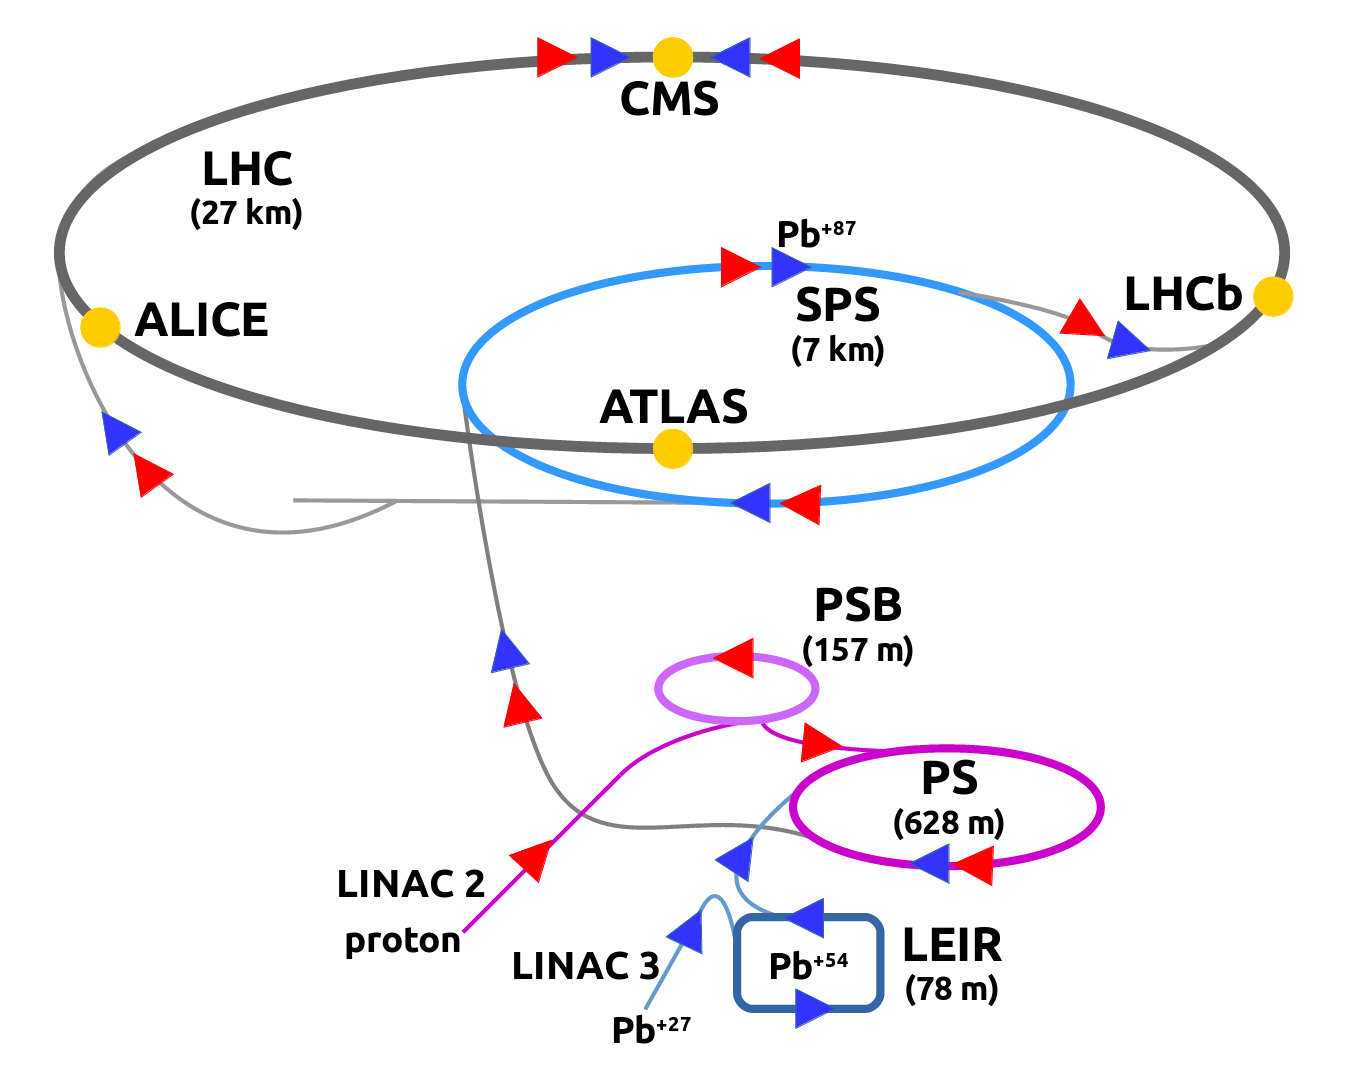
\includegraphics[width=0.7\textwidth]{Figures/Experiment/LHC/LHCInjectionChain.png}
 \caption{Schematic diagram of the LHC injection chain for protons and Pb nuclei. The proton and Pb ion trajectories are indicated with red and blue arrows, accordingly. The location of each LHC detector is also included. }
 \label{fig:LHCInjectionChain}
\end{figure}

Protons are extracted from a gas of hydrogen atoms by stripping off their electrons in a duoplasmatron, and are initially accelerated to an energy of \SI{50}{\MeV} with radio-frequency (RF) cavities in the linear accelerator Linac-2. Afterwards, they are sent to the Proton Synchrotron Booster (PSB), which is composed of four superimposed synchrotron rings that groups the protons into bunches and accelerates them to \SI{1.4}{\GeV}. Six proton bunches from the PSB are sequentially fed into the Proton Synchrotron (PS), where they are accelerated to \SI{25}{\GeV} and further splitted into 72 bunches separated in time by \SI{25}{\ns}. The proton beam is further accelerated to \SI{450}{\GeV} in the Super Proton Synchrotron (SPS) and alternately injected in the two LHC beam pipes, one beam pipe in the clockwise direction and the other in the counter-clockwise direction. Conventional electromagnets are used to keep the particles circulating in the PSB, PS and SPS accelerators.

The heavy-ion accelerator chain was initially designed in the 1990s for the SPS fixed-target experiments and then upgraded in the 2000s for the LHC. The Electron Cyclotron Resonance Ion Source (ECRIS) is used to produce heavy ions. In the case of lead, a beam of $\Pb^{27+}$ ions with an energy of 2.5~\si{\keV}/nucleon is extracted from the ECRIS every \SI{200}{\us}, and then accelerated to \SI{250}{\keV}/nucleon with a \SI{100}{\MHz} RF quadrupole (RFQ). The ion beam is sent afterwards to the linear accelerator Linac-3, which accelerates the Pb ions to \SI{4.2}{\MeV}/nucleon and transfers them to the Low Energy Ion Ring (LEIR). The $\Pb^{27+}$ ions are passed through a \SI{0.3}{\um}-thick carbon foil in the Linac-3--LEIR transfer line, stripping them to $\Pb^{54+}$ ions. The LEIR accelerates the $\Pb^{54+}$ ions to \SI{72}{\MeV}/nucleon and packs them in bunches using electron cooling. Every 3.6~s, the LEIR feeds two bunches into the PS ring and up to 16 bunches are accumulated, forming a batch, before being transferred to the SPS. The PS batch is compressed to a time interval of \SI{100}{\ns}, and accelerated to \SI{5.9}{\GeV}/nucleon. When the $\Pb^{54+}$ ions are sent to the SPS, they are fully stripped ($\Pb^{82+}$ ions) through an aluminium foil. The SPS accelerates up to twelve $\Pb^{82+}$ ion batches from the PS to \SI{176.4}{\GeV}/nucleon and then injects them into the LHC.

The LHC consists of eight straight sections called insertion regions (IR), connected by eight arc sections as shown in \fig{fig:LHCLayout}. The size and trajectory of the particle beams are controlled, in each arc section of the LHC, with a series of superconducting magnets made of Niobium-Titanium and kept at a temperature of \SI{1.9}{\K} with superfluid Helium-4. Dipole magnets are used to bend the particles, while quadrupole magnets focus the beam. Moreover, each particle beam is accelerated in IR4 with eight RF superconducting cavities operated at \SI{400}{\MHz}. The LHC beam dumping system, employed to safely stop the particle beams, is located at IR6. In addition, to protect the LHC from beam losses and absorb the beam halo, a collimation system is installed at IR3 and IR7, dedicated for beam momentum and betatron cleaning, respectively. The other four insertion regions house each of the four main LHC detectors, where the beams are collided in their corresponding interaction point (IP).

\subsection{Detectors}\label{sec:Experiment_LHC_Detectors}

The four main detectors installed in the LHC ring are:

\begin{figure}[!htbp]
 \centering
 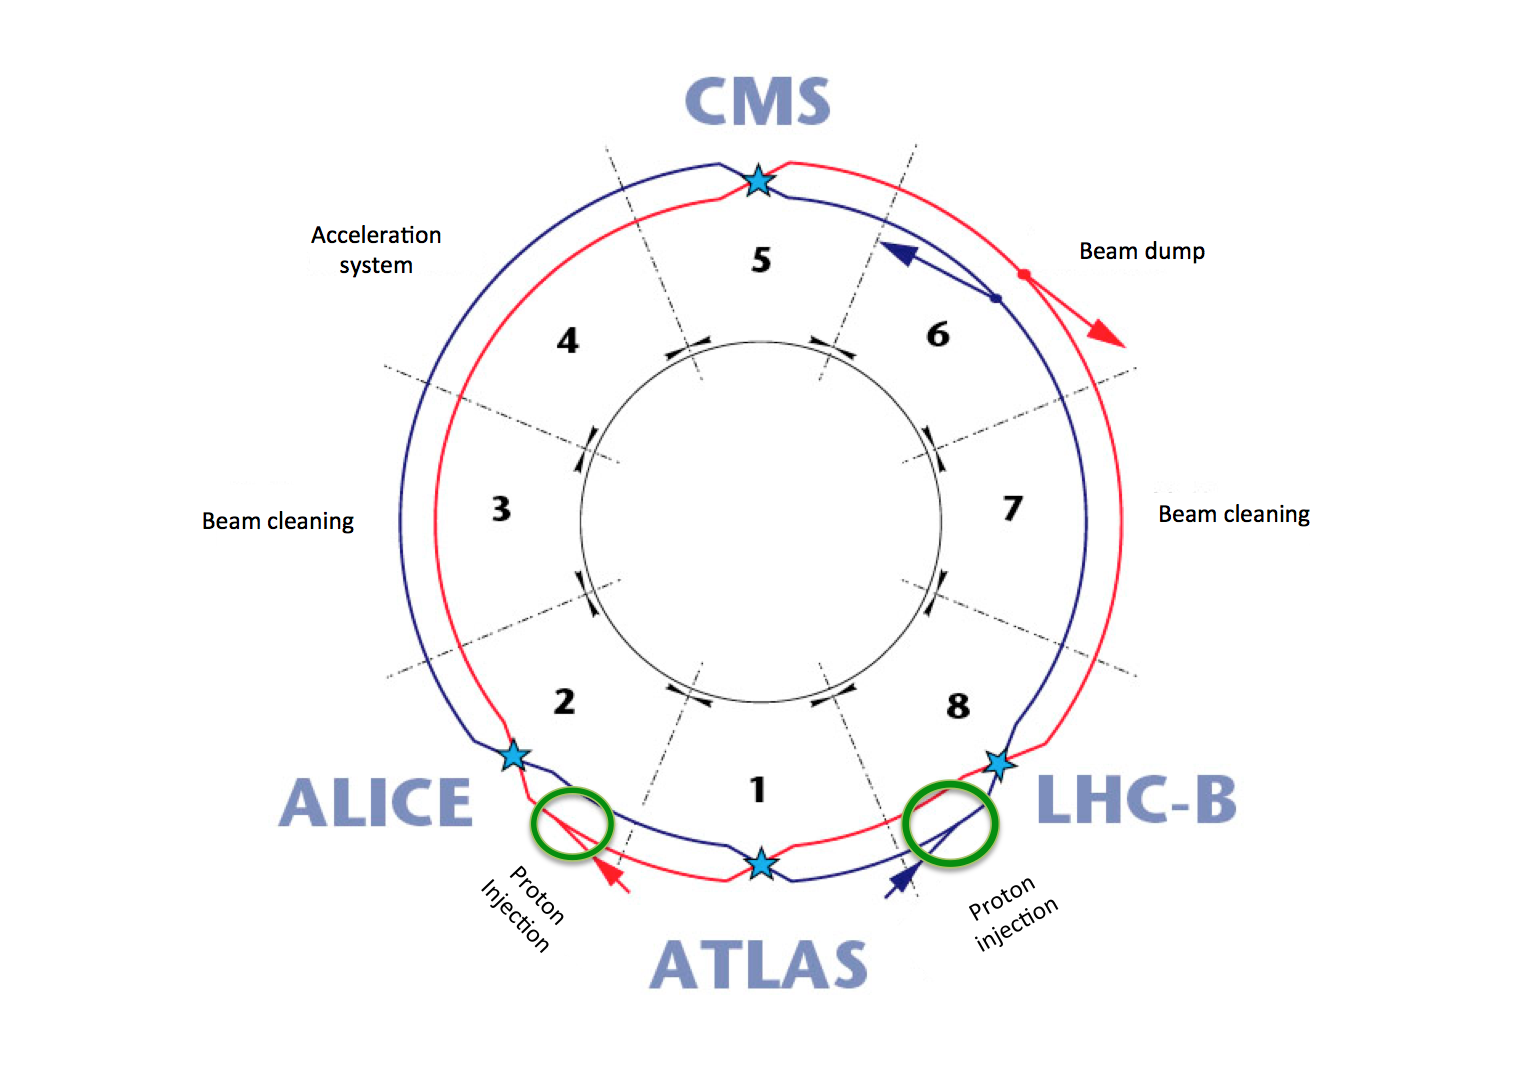
\includegraphics[width=0.8\textwidth]{Figures/Experiment/LHC/LHCLayout.png}
 \caption{Schematic diagram of the LHC layout. Figure taken from Ref.~\cite{LHCLayoutImage}.}
 \label{fig:LHCLayout}
\end{figure}

\begin{itemize}

\item A Large Ion Collider Experiment (ALICE)~\cite{ALICE}: a particle detector located at IP2, specialised on the measurement of the properties of nuclear matter at high densities. The main interest of the ALICE collaboration is the study of the QGP and the different aspects of heavy-ion physics. The ALICE detector is divided in three sets of subdetectors: the global event detectors are used to characterise the geometry of the collisions, the central barrel detectors can track charged particles down to low momentum and identify hadrons and electrons, and the muon spectrometer can reconstruct muons in the forward region.

\item A Toroidal LHC ApparatuS (ATLAS)~\cite{ATLAS}: a general-purpose particle detector located at IP1, optimised for particle collisions at the highest rates and energies achieved in the LHC. It consists of a toroidal magnetic system, an inner tracker, an electromagnetic and hadronic calorimeter, and a muon spectrometer. It is able to measure the energy of electromagnetic particles and hadrons, determine the momentum of charged particles, reconstruct jets, and identify muons with high precision. The ATLAS collaboration is involved in different physic areas including the discovery of the Higgs boson, searches for physics beyond the SM, precision measurements of electroweak and top-quark properties, and heavy-ion physics.% The ATLAS detector is fully hermetic and can cover a pseudorapidity range up to $$.

\item Compact Muon Solenoid (CMS)~\cite{CMS}: a multi-purpose particle detector located at IP5. It has a similar design as the ATLAS detector covering the same physics areas. The CMS detector and its inner components are detailed in \sect{sec:Experiment_CMS}.

\item LHCb~\cite{LHCb}: a single-arm forward spectrometer located at IP8, designed to precisely measure the decays of hadrons containing bottom quarks. It is able to distinguish between the interaction point and the b-hadron decay vertex, perform particle identification, measure the energy of electrons, photons and hadrons, and reconstruct the trajectories of charged particles. The research programme of the LHCb experiment nowadays covers heavy-flavour, QCD, electroweak and heavy-ion physics. LHCb can also operate in fixed-target mode by injecting a small amount of a noble gas (e.g. helium) around its collision region inside the beam pipe.

\end{itemize}

\subsection{Luminosity}\label{sec:Experiment_LHC_Luminosity}

The performance of the LHC can be characterised based on its delivered luminosity. The higher the luminosity of the collider, the more particle interactions occur when the beams are collided. The number of interactions per unit time $dN/dt$, produced in a given reaction, is proportional to the cross section $\sigma_{r}$ of the corresponding process, as defined in:

\begin{equation}
  \frac{dN}{dt} = {\Lumi}{\sigma_{r}}
\end{equation}

where $\Lumi$ represents the instantaneous luminosity of the particle collisions. In the case of circular beam profiles, the instantaneous luminosity depends on several factors:

\begin{equation}
  \Lumi = \frac{k_{b}N_{b,1}N_{n,2}f_{rev}{\gamma}}{4{\pi}{\epsilon_{n}}{\beta^{*}}}F
  \label{eq:Luminosity}
\end{equation}

where $k_{b}$ is the number of bunches collided, $N_{b,1}$ and $N_{b,2}$ are the number of particles per bunch in the two beams, $f_{rev} = 11245$~Hz is the revolution frequency at the LHC, $\epsilon_{n}$ is the normalised transverse beam emittance, $\beta^{*}$ is the beta-function defined at the interaction point, and $F$ is a geometric reduction factor due to the angle at which the two beams collide. The integrated luminosity is derived by integrating the instantaneous luminosity over a given period of time.

\subsection{LHC schedule}\label{sec:Experiment_LHC_Schedule}

The LHC started operations in 2008, and delivered collision data during its first running period (labelled as Run-1) until 2013, followed by a long shut-down (LS1) period of 2 years dedicated to upgrade the machine. The second period of LHC operations (Run-2) started on 2015 and will conclude at the end of 2018. During Run-1, the LHC performed proton-proton ({\Runpp}) collisions at a center-of-mass (CM) energy of $\sqrts = \SI{2.36}{\TeV}$ in 2009, and {\Runpp} collisions at $\sqrts = \SI{7}{\TeV}$ and lead-lead ({\RunPbPb}) collisions at a nucleon-nucleon CM energy of $\sqrtsnn = \SI{2.56}{\TeV}$ between 2010 and 2011. In addition, the LHC collided protons at $\sqrts = \SI{8}{\TeV}$ in 2012, and proton-lead ({\RunpPb}) at $\sqrtsnn = \SI{5.02}{\TeV}$ in 2013. Afterwards, the Run-2 period started with {\Runpp} collisions at $\sqrts = \SI{13}{\TeV}$ and {\RunPbPb} collisions at $\sqrts = \SI{5.02}{\TeV}$ in 2015, {\RunpPb} collisions at $\sqrts = \SI{8.16}{\TeV}$ in 2016, {\Runpp} collisions at $\sqrtsnn = \SI{5.02}{\TeV}$ in 2017, Xenon-Xexon ({\RunXeXe}) collisions at $\sqrtsnn = \SI{5.16}{\TeV}$, and will finish with {\RunPbPb} collisions at $\sqrtsnn = \SI{5.02}{\TeV}$ at the end of 2018.

\subsection{Heavy-ion schemes in 2015-2016}\label{sec:Experiment_LHC_Scheme}

The LHC heavy-ion physics programme began in 2010, and has since then provided data from \RunpPb and \RunPbPb collisions at various beam energies. The results presented in this thesis are based on heavy-ion data taken between 2015 and 2016. The charmonium analysis, detailed in \chp{sec:Charmonia}, uses data from \Runpp and \RunPbPb collision at $\sqrtsnn = \SI{5.02}{\TeV}$ taken in 2015, while the \Wb-boson analysis, described in \chp{sec:WBoson}, utilises \RunpPb collision data recorded in 2016.

In 2015, the LHC programme dedicated to heavy-ion physics took place during four weeks between November and December. The first week was dedicated to {\Runpp} collisions at $\sqrts = \SI{5.02}{\TeV}$ to create a reference sample for the {\RunPbPb} collision data. Each proton beam was accelerated to \SI{2.51}{\TeV}. The number of proton bunches were initially 44 and was sequentially increased during the week to a maximum of 1825 bunches. The subsequent week, the LHC beam settings were modified to collide two beams of $\Pb^{82+}$ ions at $\sqrtsnn = \SI{5.02}{\TeV}$. The LHC started accelerating ten Pb bunches to \SI{2.51}{\TeV}/nucleon, and then progressively increased the number of Pb bunches until it reached 518 at the end of the \RunPbPb data taking. The Pb beam lifetime was shorter than for protons due to the large ultraperipheral electromagnetic interactions between Pb ions, requiring to refill the beams more often. All experiments took \RunPbPb collision data, including LHCb for the first time~\cite{LHCPbPb2015}. The integrated luminosity of the {\RunPbPb} collision data is shown in the left plot of \fig{fig:LHCPbPb2015}.

\begin{figure}[!htbp]
 \centering
 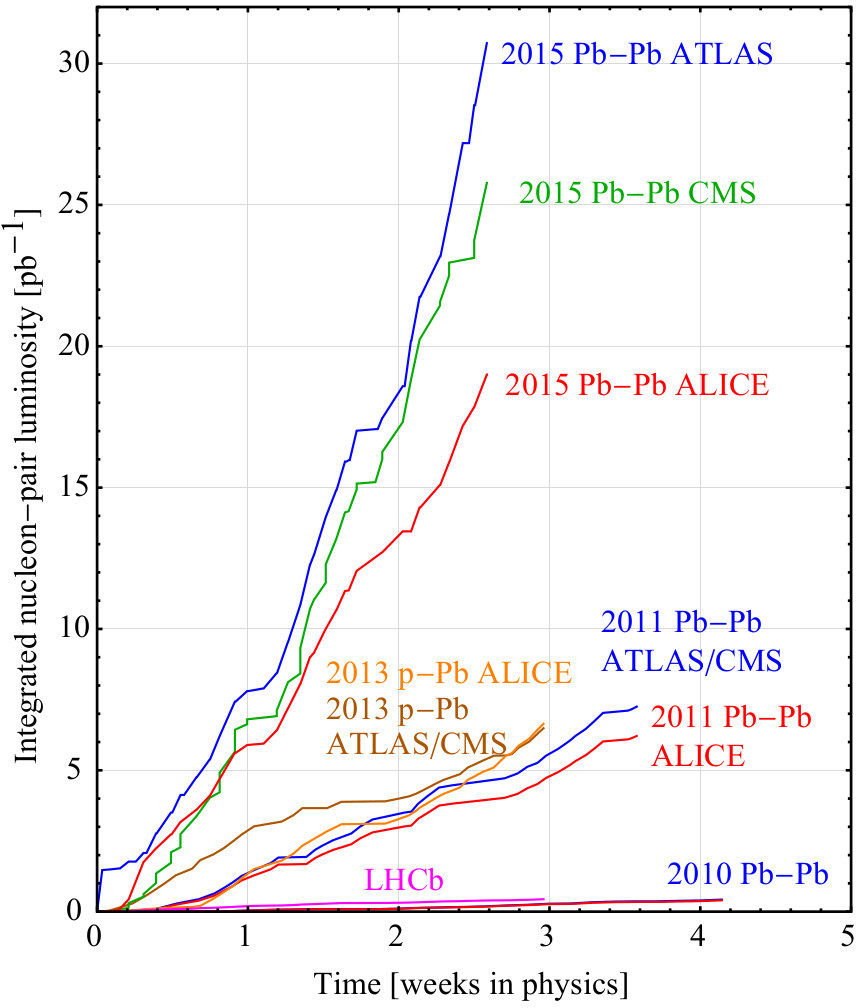
\includegraphics[width=0.4\textwidth]{Figures/Experiment/LHC/PbPb2015Lumi.png}
 \caption{Integrated nucleon-pair luminosity delivered by the LHC to each experiment during \RunPbPb collisions at $\sqrtsnn = \SI{5.02}{\TeV}$. The integrated luminosity of \RunpPb collisions at $\sqrtsnn = \SI{5.02}{\TeV}$ and \RunPbPb collisions at $\sqrtsnn = \SI{2.76}{\TeV}$ are included for comparison. Figure taken from Ref.~\cite{LHCPbPb2015}. }
 \label{fig:LHCPbPb2015}
\end{figure}

The following year, asymmetric collisions of $\Pb^{82+}$ nuclei with protons were performed between November 7th and December 4th. Several beam configurations were implemented in 2016 to fulfil the interests of each experiment: ALICE requested {\RunpPb} data at $\sqrtsnn = \SI{5.02}{\TeV}$, CMS and ATLAS asked for {\RunpPb} data at $\sqrtsnn = \SI{8.16}{\TeV}$ with an integrated luminosity of at least $\Lumi = 100$~\nbinv, and LHCb requested {\RunpPb} collisions at $\sqrtsnn = \SI{8.16}{\TeV}$ complemented with a reversal of the beam direction. After careful planning, the first ten days were dedicated to {\RunpPb} collisions at $\sqrtsnn = \SI{5.02}{\TeV}$ optimised for ALICE. Afterwards, the LHC spent two weeks on {\RunpPb} collisions at $\sqrtsnn = \SI{8.16}{\TeV}$. At the beginning of the  {\RunpPb} collisions at $\sqrtsnn = \SI{8.16}{\TeV}$, the proton beam was composed of 702 bunches at \SI{6.5}{\TeV} moving in the clockwise direction, while the Pb beam was made of 548 bunches at \SI{2.56}{\TeV}/nucleon moving in the anti-clockwise direction, around the LHC rings. The LHC then proceeded to reverse the beam directions after the integrated luminosity accumulated in CMS and ATLAS reached half of the requested value ($\sim{60~\nbinv}$), and kept colliding 540 Pb bunches with 684 proton bunches during the last nine days. At the end of the heavy-ion data taking period, the LHC managed to deliver a total integrated luminosity of $\Lumi = 188$~\nbinv of \RunpPb data to the CMS experiment as shown in \fig{fig:LHCpPb2016}. The beam settings used by LHC during the heavy-ion collision programme performed in 2015 and 2016 are summarised in \tab{tab:LHCScheme}.

\begin{figure}[!htbp]
 \centering
 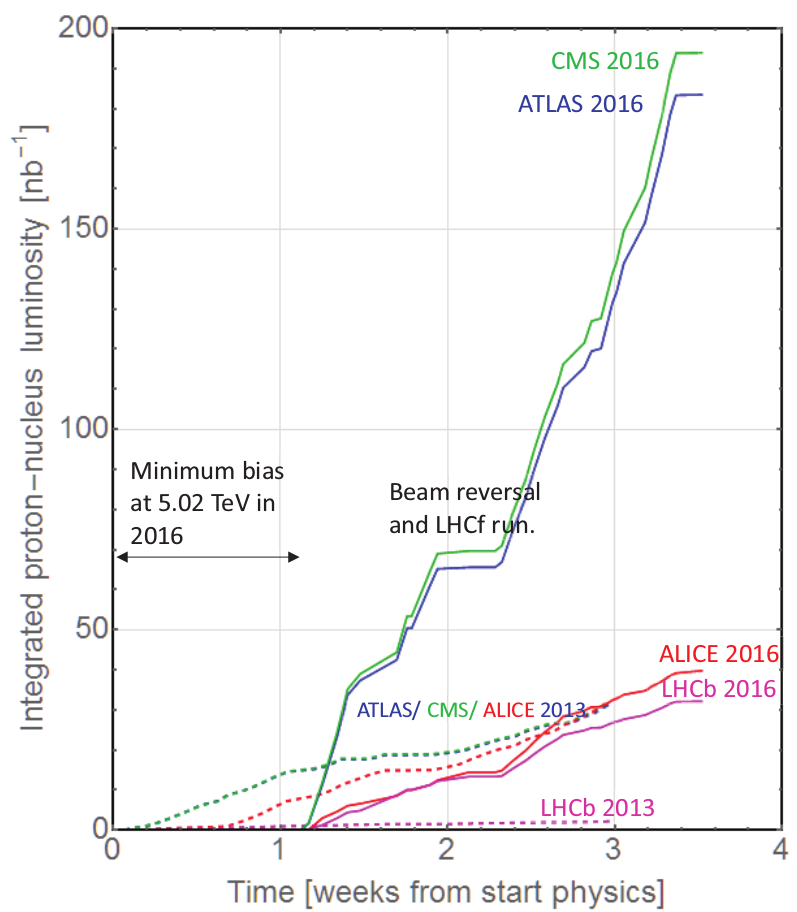
\includegraphics[width=0.4\textwidth]{Figures/Experiment/LHC/ProtonLead2016Lumi.png}
 \caption{Integrated proton-nucleus luminosity delivered by the LHC to each experiment during \RunpPb collisions at $\sqrtsnn = \SI{8.16}{\TeV}$ (solid lines). The integrated luminosity of \RunpPb collisions at $\sqrtsnn = \SI{5.02}{\TeV}$ (dashed lines) is included for comparison. Figure taken from Ref.~\cite{LHCpPb2016}. }
 \label{fig:LHCpPb2016}
\end{figure}

\begin{table}[!htbp]
 \centering
 \begin{tabular}{ c c c c }
   Variable & \Runpp 2015 & \RunPbPb 2015 & \RunpPb 2016 \\
   \hline
   Fill no. & 4647 & 4720 & 5562 \\
   Collision energy $\sqrtsnn$ $\left[\si{\TeV}\right]$ & 5.02 & 5.02 & 8.16 \\
   Pb beam energy $E_{\Pb}$ $\left[\si{\TeV}/\text{nucleon}\right]$ & - & 2.51 & 2.56 \\
   Beam energy $E_{\Pp}$ $\left[\si{\TeV}/\text{proton}\right]$ & 2.56 & 6.37 & 6.5 \\
   Pb ions per bunch $N^{\Pb}_{b}$ $\left[10^{8}\right]$ & - & 2.0 & 2.1 \\
   Protons per bunch $N^{\Pp}_{b}$ $\left[10^{10}\right]$ & 10.1 & - & 2.7 \\
   No. of Pb bunches $k^{\Pb}_{b}$ & - & 518 & 540 \\
   No. of proton bunches $k^{\Pp}_{b}$ & 1825 & - & 684 \\
   No. of colliding bunches $k_{c}$ & 1813 & 491 & 513 \\
   $\beta^{*}$ $\left[\si{\meter}\right]$ & 4 & 0.8 & 0.6 \\
   Crossing angle $\left[\si{\micro\radian}\right]$ & 170 & 145 & 140 \\
   Pb beam emittance $\epsilon^{\Pb}_{n}\left(x,y\right)$ $\left[\si{\um}\right]$ & - & 2.1 & 1.6 \\
   Pb bunch length $\sigma^{\Pb}_{z}$ $\left[\si{\meter}\right]$ & - & 0.09 & 0.9 \\
   CMS peak lumi. $\Lumi^{peak}$ $\left[10^{27}~\si{\per\cm\squared\per\s}\right]$ & $3.4{\times}10^{5}$ & 3 & 869 \\
   CMS integrated lumi. $\Lumi_{int}$ $\left[\nbinv\right]$ & 28820 & 0.6 & 188 \\
 \end{tabular}
 \caption{LHC beam parameters during the highest luminosity physics fills. The luminosity values are averages for CMS. Information extracted from Ref.~\cite{LHCScheme}. }
 \label{tab:LHCScheme}
\end{table}


\section{The Compact Muon Solenoid}\label{sec:Experiment_CMS}

The CMS~\cite{CMS} is a multi-purpose particle detector housed in an underground cavern at IP5 of the LHC. The CMS experiment is integrated, at the time of writing this thesis, by an international collaboration of over 5600 members from around 215 institutes from 46 countries. The CMS is composed of a central barrel in the mid-rapidity region closed by two endcap disks, one on each side of the IP, forming a hermetic cylindrical detector. The CMS detector consists of four main subdetector systems: the silicon tracker, the Electromagnetic CALorimeter (ECAL), the Hadronic CALorimeter (HCAL) and the muon chambers. A superconducting solenoid magnet placed in the barrel section generates a magnetic field of \SI{3.8}{\tesla}. The tracking system, the ECAL and the HCAL, are located within the solenoid volume, while the muon system is placed between the layers of the flux-return yoke, which confines the magnetic flux. A sectional view of the CMS detector including the number of channels per subdetector, in its 2016 configuration, is shown in \fig{fig:CMS2016}.

\begin{figure}[!htbp]
 \centering
 \includegraphics[width=1.0\textwidth]{Figures/Experiment/CMS/CMS.pdf}
 \caption{Cutaway view of the CMS detector in its configuration used during 2015 and 2016. Labels and basic details of each subdetector are included.~\cite{CMSLayout} }
 \label{fig:CMS2016}
\end{figure}

One of the main components of the CMS detector is its superconducting solenoid magnet of \SI{6}{\m} internal diameter and \SI{12.5}{\m} length. The magnet produce a uniform magnetic field of \SI{3.8}{\tesla} in the central region by supplying an electric current of \SI{18.1}{\kA} through a four-layer winding coil made of NbTi wire. To be able to sustain the large electric currents, the solenoid coil is thermally insulated within a vacuum volume and operated in superconducting mode at a temperature of \SI{4.6}{\K} with a thermal-siphon cooling system fed with liquid helium. The flux of the magnetic field outside the barrel is returned through a massive steel yoke of 10000 tons divided in five barrel wheels and four endcap disks at each end. In case there is a major system fault or the magnet suffers a superconducting-to-resistive transition (quench), the electric power source is immediately disconnected and the stored magnetic energy is quickly discharged through a \SI{30}{\mohm} dump resistor placed outdoors.

The coordinate system of the CMS detector is centred at the interaction point. It is oriented in such a way that the $x$-axis points radially inward to the centre of the LHC ring while the $y$-axis points upward perpendicular to the LHC plane. The $z$-axis is defined parallel to the beam. By convention, the positive $z$-direction is defined along the counter-clockwise beam direction. For asymmetric collisions, such as \RunpPb, it is later reversed (if necessary) to match the proton-going direction, so that the "forward" (low Bjorken-x) physics corresponds to the "forward" ($\eta > 0$) part of the detector (see \sect{sec:WBoson_Analysis_Samples_Data}).

The trajectory of particles measured at CMS is described in the coordinate system displayed in \fig{fig:CMSCoordinates}. The polar angle $\theta$ is measured from the $z$-axis while the azimuthal angle $\phi$ is measured from the $x$-axis in the $x$-$y$ plane, called the transverse plane. The radial coordinate $r$ is also measured in the transverse plane. The polar angle is replaced by the pseudorapidity $\eta$ which, for massless particles, matches the rapidity and is Lorentz invariant under longitudinal boosts. The pseudorapidity is zero in the transverse plane and approaches infinity towards to the $z$-axis, according to:

\begin{equation}
  \eta = -\ln\left[\tan\left(\frac{\theta}{2}\right)\right]
\end{equation}

\begin{figure}[!htbp]
  \centering
  % CMS conventional coordinate system with LHC and other detectors
  \tdplotsetmaincoords{75}{50} % to reset previous setting
  \begin{tikzpicture}[scale=2.7,tdplot_main_coords,rotate around x=90]
 
  % variables
  \def\rvec{1.2}
  \def\thetavec{40}
  \def\phivec{70}
  \def\R{1.1}
  \def\w{0.3}
 
  % axes
  \coordinate (O) at (0,0,0);
  \draw[thick,->] (0,0,0) -- (1,0,0) node[below left]{$x$};
  \draw[thick,->] (0,0,0) -- (0,1,0) node[below right]{$y$};
  \draw[thick,->] (0,0,0) -- (0,0,1) node[below right]{$z$};
  \tdplotsetcoord{P}{\rvec}{\thetavec}{\phivec}
 
  % vectors
  \draw[->,red] (O) -- (P) node[above left] {$P$};
  \draw[dashed,red] (O)  -- (Pxy);
  \draw[dashed,red] (P)  -- (Pxy);
  \draw[dashed,red] (Py) -- (Pxy);
 
  % circle - LHC
  \tdplotdrawarc[thick,rotate around x=90,black!70!blue]{(\R,0,0)}{\R}{0}{360}{}{}
 
  % compass - the line between CMS and ATLAS has a ~12° declination (http://googlecompass.com)
  \begin{scope}[shift={(1.1*\R,0,1.65*\R)},rotate around y=12]
    \draw[<->,black!50] (-\w,0,0) -- (\w,0,0);
    \draw[<->,black!50] (0,0,-\w) -- (0,0,\w);
    \node[above left,black!50,scale=0.6] at (-\w,0,0) {N};
  \end{scope}
 
  % nodes
  \node[right] at (\R,0,0) {LHC};
  \fill[radius=0.8pt,black!20!red]
    (O) circle node[left=4pt,below=2pt] {CMS};
  \draw[thick] (0.02,0,0) -- (0.5,0,0); % partially overdraw x-axis and CMS point
 
  % arcs
  \tdplotdrawarc[->]{(O)}{0.2}{0}{\phivec}
    {above=2pt,right=-1pt,anchor=mid west}{$\phi$}
  \tdplotdrawarc[->,rotate around z=\phivec-90,rotate around y=-90]{(0,0,0)}{0.5}{0}{\thetavec}
    {anchor=mid east}{$\theta$}
 
  \end{tikzpicture}
  \caption{Schematic diagram of the coordinate system used in the CMS experiment.}
  \label{fig:CMSCoordinates}
\end{figure}


The details of the original configuration of the CMS detector can be found in Ref.~\cite{CMS}. After Run-1 was over, the CMS underwent several improvements as part of the planned upgrades for the LS1 shut-down period (2013-2014). The systems upgraded during LS1 include the muon endcap stations, the hadron calorimeter, and the L1 trigger. In the case of the muon system, an additional disk of muon detectors was installed on the outermost part of each endcap section providing a fourth measurement in the forward region~\cite{CMSMuonUpgrade}. Moreover, the photosensors of the forward (outer-barrel) hadron calorimeter were replaced with multi-anode photomultiplier tubes (silicon photomultipliers), and the corresponding readout electronics were upgraded to handle the new sensors~\cite{CMSHCALUpgrade}. And finally, the framework and electronics of the L1 trigger system were completely changed to sustain the increasing interaction rate of the LHC beam collisions~\cite{L1_Stage2}.


\subsection{Subdetectors}\label{sec:Experiment_CMS_Subdetectors}

The CMS detector~\cite{CMS} is composed of several subdetectors which provide a precise measurement of the trajectory and energy of the particles emitted from the LHC collisions. The superconducting solenoid volume contains the inner tracker close to the beam line followed radially outwards by the electromagnetic and hadronic calorimeters. The muon chambers are installed outside of the solenoid, interspersed with layers of the flux-return yoke. An electromagnetic preshower is installed in the endcaps complementing the ECAL to improve the identification of photons and electrons.


\subsubsection{Tracker}\label{sec:Experiment_CMS_Subdetectors_Tracker}

The CMS tracking system is designed to measure the trajectory of charged particles and reconstruct the 3D vertex position of the primary interaction and the secondary decays. It is completely surrounded by the volume of the solenoid magnet in the barrel region, and has a diameter of \SI{2.5}{\m} and a length of \SI{5.8}{\m}, centred on the interaction point. The CMS tracker is made of a pixel detector and a silicon strip tracker. A schematic cross section of the CMS tracker is presented in \fig{fig:CMS_Tracker}.

\begin{figure}[!htbp]
 \centering
 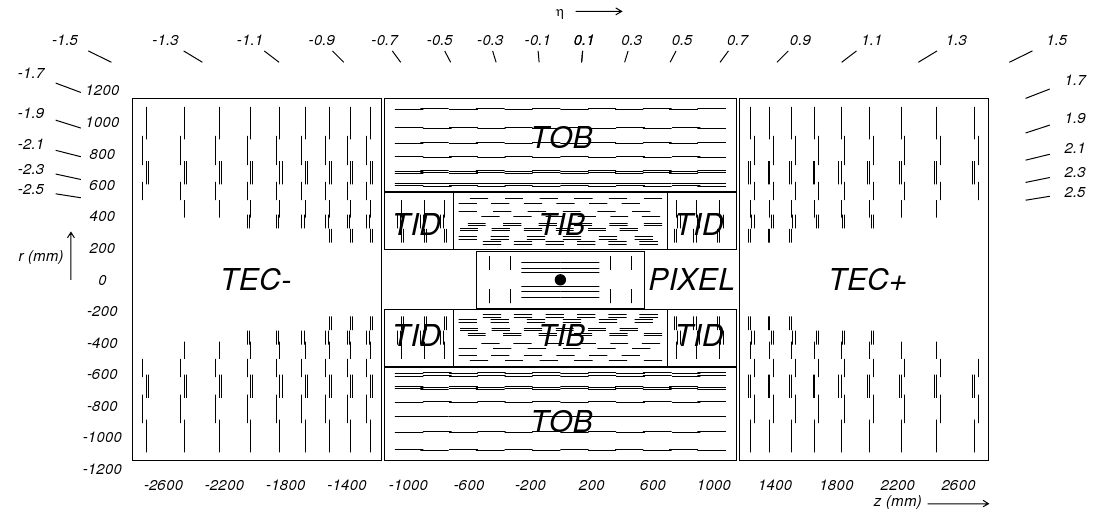
\includegraphics[width=1.0\textwidth]{Figures/Experiment/CMS/Tracker.png}
 \caption{View of the CMS tracker in the $r$-z plane. Each line represents a detector module. Figure taken from Ref.~\cite{CMS}.}
 \label{fig:CMS_Tracker}
\end{figure}

The pixel detector is made of 1440 pixel modules installed in the tracker section closest to the interaction region. It covers the pseudorapidity range $|\eta|<2.5$ with three Barrel Pixel (BPix) layers and two Forward Pixel (FPix) disks. The BPix layers are placed at a radii of \SI{4.4}{\cm}, \SI{7.3}{\cm} and \SI{10.2}{\cm} from the beam axis, while the FPix disks are located, on each side of the IP, at a longitudinal distance of $z={\pm}\SI{34.5}{\cm}$ and $z={\pm}\SI{46.5}{\cm}$. The BPix (FPix) detectors contain 48 (18) million silicon pixels, each with a cell size of $100{\times}\SI{150}{\um\squared}$. The arrangement of the pixel detector modules in the barrel (forward) region provides, over the full tracker coverage, three tracking hits per track and a position resolution of 15-20 (15)~\si{\um} in the $z$-coordinate.

The silicon-strip tracker contains 9.3 million strips divided in 24244 silicon sensors, covering the region between the pixel detector and the ECAL. In the barrel region, the strip tracker is composed of the Tracker Inner Barrel (TIB), made of four concentric cylinders placed at a radius between \SI{25.5}{\cm} and \SI{49.8}{\cm}, and the Tracker Outer Barrel (TOB), which consists of a wheel-like structure containing six cylinders with an inner (outer) radius of 55.5 (116)~\si{\cm}. The pseudorapidity coverage of the strip tracker is extended up to $|\eta|=2.5$ with three Tracker Inner Disks (TID) and nine Tracker EndCap (TEC) disks, installed on each endcap section along $\SI{80}{\cm} < |z| < \SI{90}{\cm}$ and $\SI{124}{\cm} < |z| < \SI{282}{\cm}$, accordingly. The strip detector modules used in the TIB, TID and inner four TEC rings are made of one \SI{320}{\um}-thick sensor, while those used in the TOB and outer five TEC rings are made of two \SI{500}{\um}-thick sensors. The strip pitch varies between 80-\SI{120}{\um}, 100-\SI{141}{\um}, 122-\SI{183}{\um}, and 97-\SI{184}{\um}, in the TIB, TID, TOB and TEC, respectively. The strip tracker can achieve a position resolution in the TIB (TOB) of 23-35 (35-53)~\si{\um} in the transverse plane and 230 (530)~\si{\um} in the $z$-coordinate.


\subsubsection{Electromagnetic calorimeter}\label{sec:Experiment_CMS_Subdetectors_ECAL}

The ECAL of the CMS is a hermetic homogeneous calorimeter composed of 75848 lead-tungstate ($\text{PbWO}_{4}$) crystals. The ECAL is designed to fully absorb and measure the energy of electrons and photons. The $\text{PbWO}_{4}$ material was chosen for its small Moli{\`e}re radius (\SI{2.2}{\cm}), a short radiation length (\SI{0.89}{\cm}), and a high density (\SI{8.28}{\gram\per\cm\cubed}). When a high-energy electron or photon interacts with the nuclei of the ECAL crystals, it generates a cascade of electromagnetic particles ($e^{-}$, $e^{+}$ and $\gamma$) and induces the emission of blue scintillation light ($\lambda\approx\SI{420}{\nm}$), which is then measured in photodetectors. The total amount of scintillation light produced is proportional to the energy deposited in the crystals by the electrons and photons. In order to cope with the running conditions of the LHC, the crystals are designed to have a fast response (\SI{25}{\ns}), and be optically transparent and radiation-hard.

The ECAL is installed between the silicon-strip tracker and the HCAL. It is divided in a cylindrical-barrel section (EB) and two endcap rings (EE), one on each side of the IP. The EB is made of 61200 crystals of \SI{23}{\cm} long, covering the pseudorapidity range $|\eta|<1.48$ with a granularity of 170-fold in $\eta$ and 360-fold in $\phi$. The crystals are grouped in modules of either 400 or 500 units, and four modules are assembled in so-called supermodules. The EB has a total of 36 supermodules, each covering \ang{20} in $\phi$ with 1700 crystals. The scintillation light is measured in the EB with Avalanche PhotoDiodes (APD), mounted in pairs on the back of each crystal. Each APD is operated, with a high-voltage power supply system, at gain 50 and a voltage between 340-\SI{430}{\V}. The schematic layout and geometric view of the ECAL are shown in \fig{fig:CMS_ECAL}.

\begin{figure}[!htbp]
 \centering
 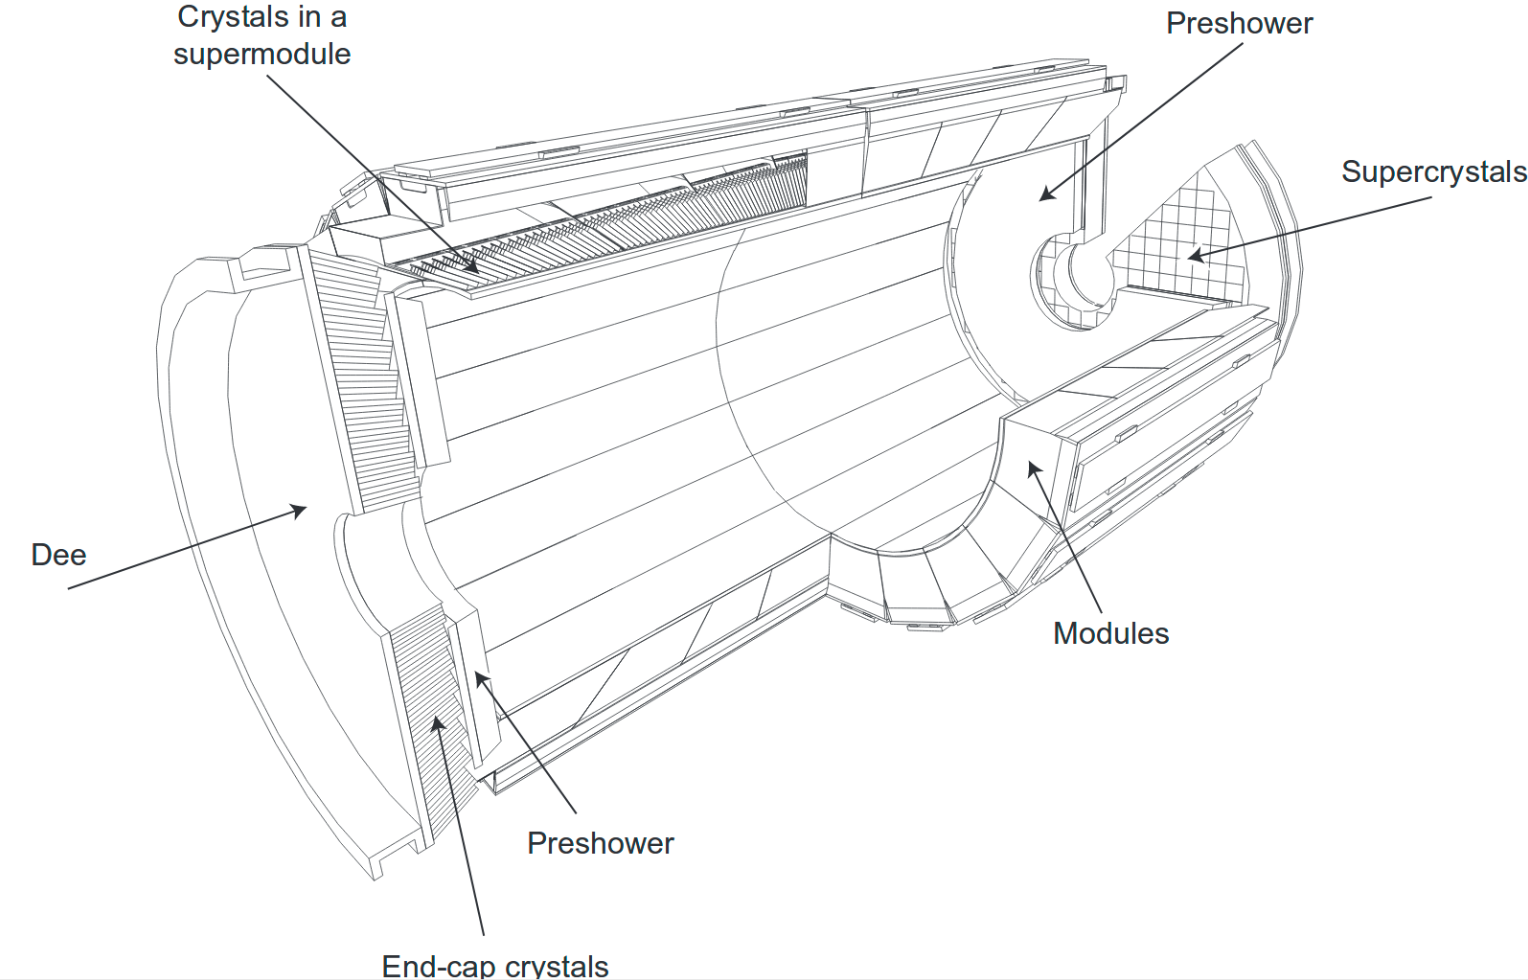
\includegraphics[width=0.43\textwidth]{Figures/Experiment/CMS/ECALLayout_1.png}
  %
 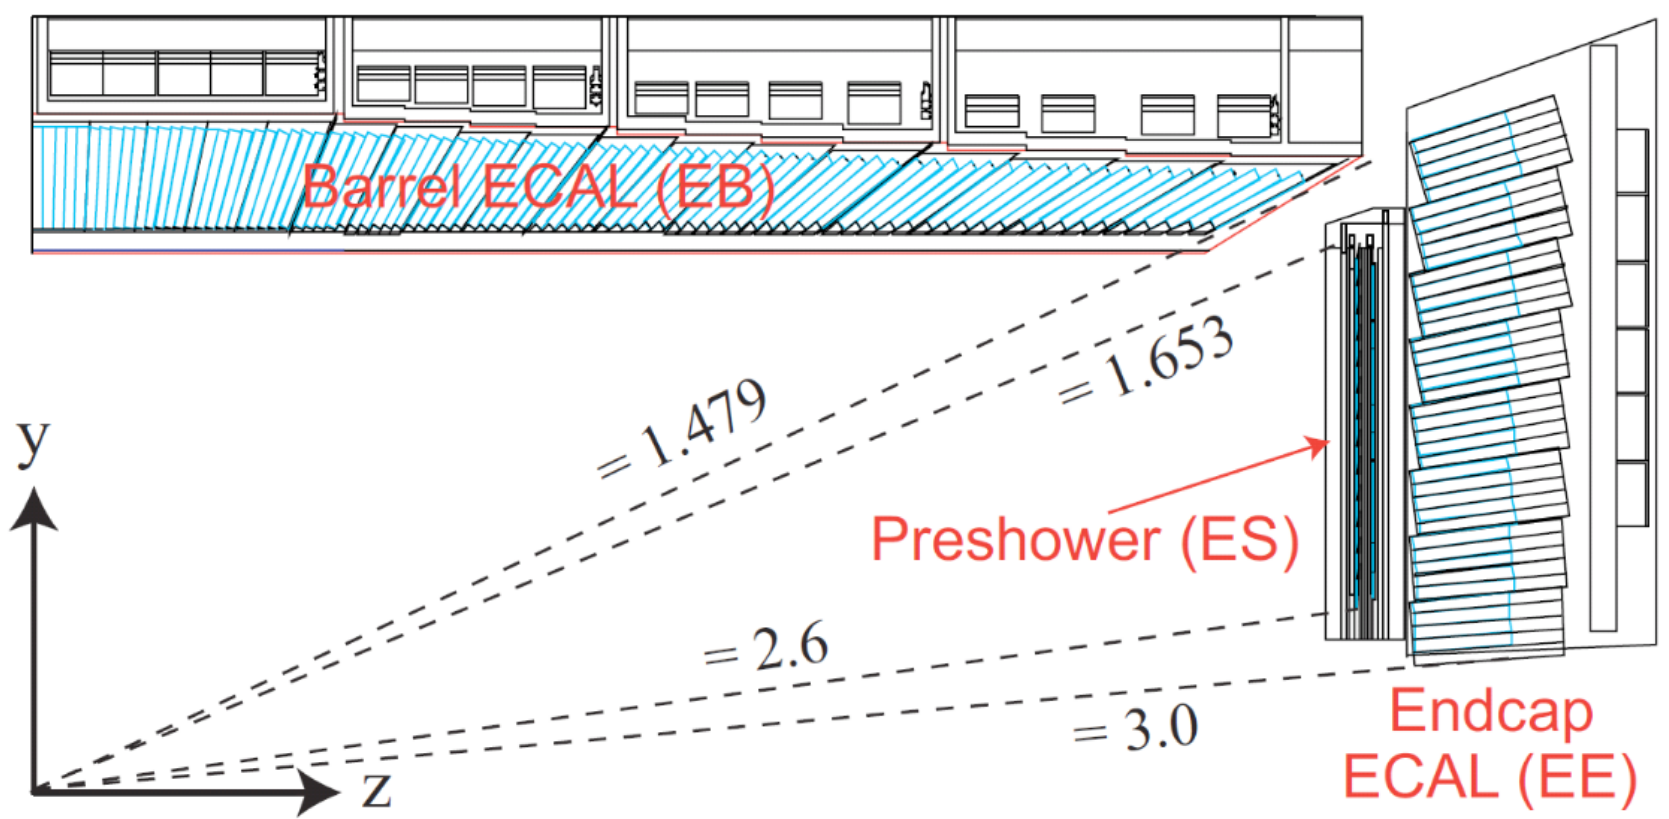
\includegraphics[width=0.53\textwidth]{Figures/Experiment/CMS/ECALLayout_2.png}
 \caption{Schematic layout~\cite{CMS} (left) of the CMS electromagnetic calorimeter, and its corresponding one-quarter geometric view~\cite{CMSECAL} (right).}
 \label{fig:CMS_ECAL}
\end{figure}

The EE rings are installed at $z = {\pm}\SI{3.15}{\m}$, extending the coverage of the ECAL up to $|\eta| = 3.0$. The EE consists of 14648 crystals of \SI{22}{\cm} long, assembled in units of $5{\times}5$ crystals known as SuperCrystals (SC). Each EE ring is divided in two halves, each containing 156 SCs. A single-stage photomultiplier called Vacuum PhotoTriodes (VPT), attached to the back of each EE crystal, is used to measure the scintillation photons. The VPT has a diameter of \SI{25}{\mm}, a quantum efficiency of $22\%$ at a wavelength of \SI{430}{\nm}, and a gain of 10.2 at zero magnetic field.

An additional calorimeter called the Preshower detector is installed in the endcap rings between the tracker and the EE. The Preshower is an electromagnetic sampling calorimeter of \SI{20}{\cm} thickness,  optimised to identify photons from neutral pion decays. It is composed of two layers of lead absorbers interleaved with 4300 silicon sensors organised in 32 strips. Each silicon sensor has a thickness of \SI{320}{\um} and an active area of $63{\times}\SI{63}{\mm\squared}$. Incoming photons and electrons initiate an electromagnetic shower when they interact with the lead absorbers. The energy deposited in the absorbers and the transverse profile of the shower are measured in the silicon strips.

The response of the crystals and the signal amplification of the APDs depend on the operating temperature. As a result, a water flow cooling system is installed to keep the crystals and sensors at a stable  temperature of $18.00\pm\SI{0.05}{\celsius}$. Moreover, the transparency of the crystals to scintillation light is affected by the radiation dose due to the formation of colour centres which absorbs part of the light. The variation of the crystal transparency is monitored using laser pulses introduced into the crystals at a frequency of \SI{80}{\Hz}. The laser monitoring system uses two blue lasers ($\lambda\approx\SI{440}{\nm}$) to track the radiation-induced transparency variations, which are then corrected for by recalibrating the detector.

The energy resolution of the ECAL is affected by several sources, such as the fluctuations in the shower, crystal non-uniformities, calibration errors, and noise in the photodetectors. The relative energy resolution of the ECAL is parametrised as a function of the measured energy $E$ via:

\begin{equation}
  \left(\frac{\sigma_{E}}{E}\right)^{2} = \left(\frac{2.8\%}{\sqrt{E/\si{\GeV}}}\right)^{2} + \left(\frac{12\%}{E/\si{\GeV}}\right)^{2} + \left(0.3\%\right)
\end{equation}


\subsubsection{Hadronic calorimeter}\label{sec:Experiment_CMS_Subdetectors_HCAL}

The HCAL is a hermetic sampling calorimeter made of 70000 plastic-scintillator tiles interleaved with absorber plates. The goal of the HCAL is to completely absorb and measure the energy of hadrons. When a hadron hits an absorber plate, it induces a shower of particles through the successive absorber layers. The secondary particles produced in the cascade pass through the plastic tiles, located in between the absorbers, leading to the emission of scintillator light at a peak wavelength of $\sim\SI{440}{\nm}$. Photons generated on each tile are collected with WaveLength-Shifting (WLS) fibres fabricated in a double-clad configuration with a diameter of \SI{0.94}{\mm}. The WLS fibres shifts the scintillator light to the green spectrum (\SI{515}{\nm}) and pass it to fibre-optic waveguides which then transfers the light to a phototransducer. The scintillator tiles are grouped in trays that are \ang{5} wide in $\phi$. A geometric view of CMS, highlighting the different components of the HCAL, is presented in \fig{fig:CMS_HCAL}.

\begin{figure}[!htbp]
 \centering
 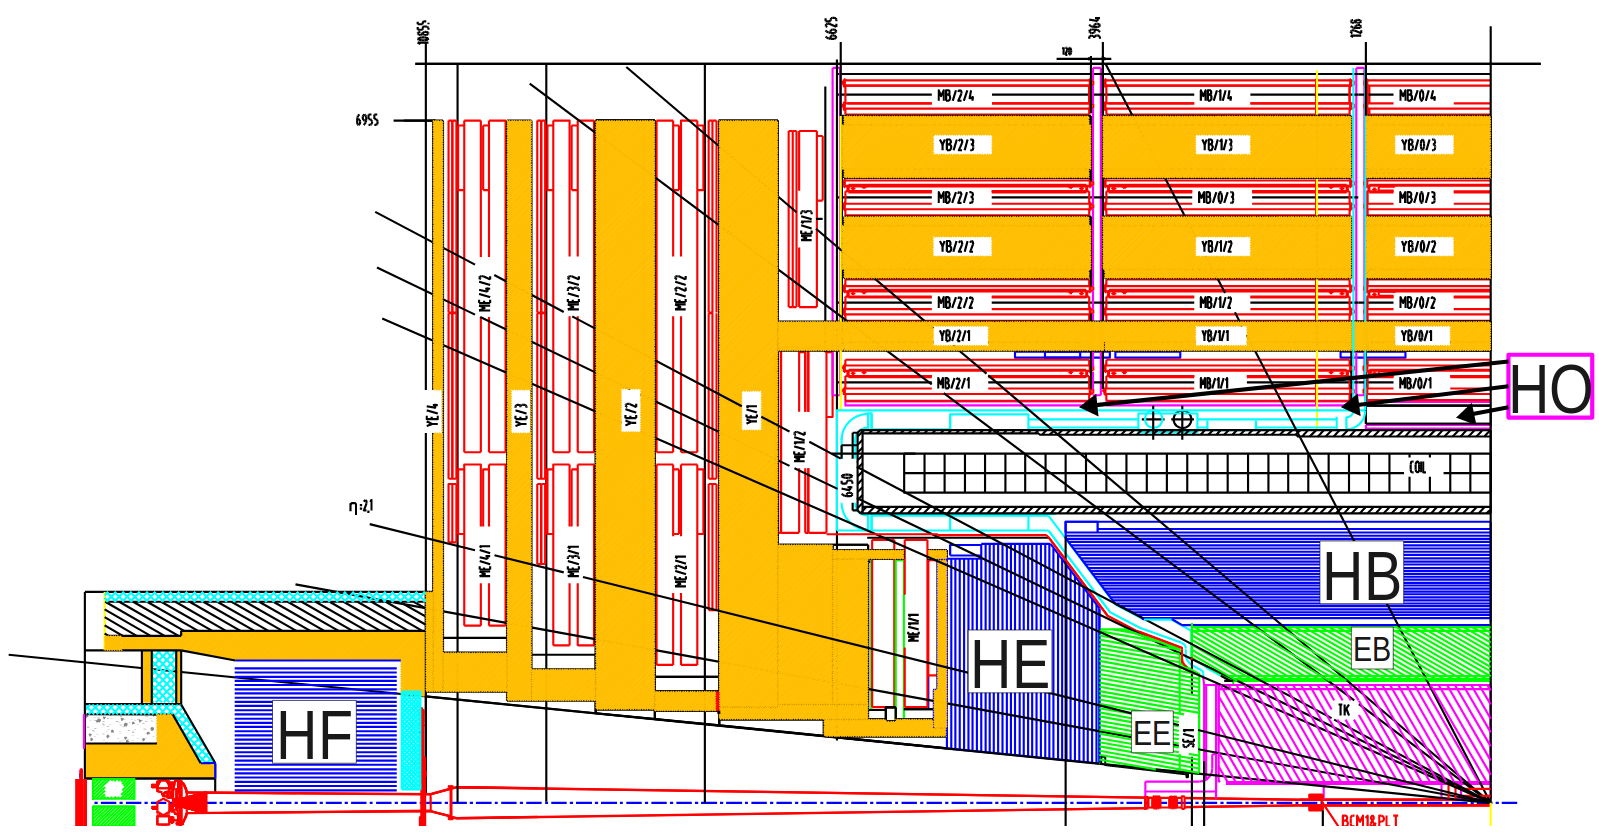
\includegraphics[width=0.9\textwidth]{Figures/Experiment/CMS/HCAL.png}
 \caption{Geometric view of one quarter of the CMS detector, displaying the subdetectors of the hadron calorimeter: HB, HE, HF and HO. Figure taken from Ref.~\cite{CMSHCALUpgrade}.}
 \label{fig:CMS_HCAL}
\end{figure}

The central region of the HCAL is composed of the Hadron-Barrel (HB) calorimeter installed between the ECAL and the magnet coil, and the Hadron-Outer (HO) calorimeter placed outside of the solenoid volume. The HB covers the pseudorapidity range $|\eta| < 1.3$, and it is divided in two half-barrel sections. The absorber consists of 36 wedges of brass and steel plates aligned parallel to the z-axis. Each HB wedge is splitted in four azimuthal sections. The HB scintillator tiles are divided in 16 $\eta$-parts providing a $\Delta\eta{\times}\Delta\phi$ segmentation of $0.087{\times}0.087$. The HB photosensors consist of  Hybrid PhotoDiode (HPD) transducers. The HPD contains 19 pixels of \SI{20}{\mm\squared} in size and has an approximate gain of 2000.

The HO is used to measure the energy of the tail of the particle shower deposited after the HB. The HO is divided in five disks corresponding to each of the five barrel wheels of the flux-return yoke. Each HO ring is divided into twelve $\phi$ sectors, each separated in six trays. The HO has 2730 scintillator tiles of \SI{10}{\mm} thick organised in 422 trays, offering the same $\Delta\eta{\times}\Delta\phi$ granularity as the HB. The HO uses a multipixel Geiger-mode APD, known as Silicon PhotoMultiplier (SiPM), to detect photons.

The coverage of the HCAL is extended in the forward region to $|\eta| = 3$ with the Hadron-Endcap (HE) calorimeter and up to $|\eta| = 5.2$ with the Hadron-Forward (HF) calorimeter. The HE is located in the endcap rings and its absorber is made of two \SI{79}{\mm}-thick plates of cartridge brass separated by \SI{9}{\mm}. The HE contains 20916 plastic tiles and has a $\Delta\eta{\times}\Delta\phi$ granularity of  $0.17{\times}0.17$. The HE also uses HPDs to measure the scintillator light.

The HF is divided in 36 wedges that are \ang{20} wide in $\phi$, and its front face is located at $z = {\pm}\SI{11.2}{\m}$, on each side of the IP. Since the HF experience a large energy deposit from the beam collisions, its design has been optimised to handle high levels of radiation. The HF absorber consists of a \SI{1.7}{\m}-depth cylindrical structure made of \SI{5}{\mm}-thick steel-grooved plates, while the HF active medium is composed of quartz fibres of polymer hard-cladding and fused-silica core. The signal consists of Cherenkov light generated when energetic charged particles from the shower traverse the quartz fibres. The Cherenkov light is measured by  multi-anode PhotoMultiplier Tubes (PMT) shielded behind \SI{40}{\cm} of steel. The HF fibres are inserted in the absorber grooves along the beam line in two longitudinal segments. Long fibres are inserted over the full absorber depth while short fibres starts at a depth of \SI{22}{\cm} from the front face covering the back of the absorber. Since most of the energy of electrons and photons is deposited in the first \SI{22}{\cm} while hadrons are able to penetrate more in the HF absorber, the difference in energy measured in the long and short fibres is used to estimate the electromagnetic and hadronic components of the shower.


\subsubsection{Muon detectors}\label{sec:Experiment_CMS_Subdetectors_Muon}

The CMS muon tracking system measures the momentum and charge of muons in the fiducial region $|\eta| < 2.4$. It is divided in four stations corresponding to four concentric cylinders in the barrel region and to four disks on each endcap section. \fig{fig:CMS_Muon} shows a geometric view of one quadrant of the CMS muon system. The dense material of the calorimeters and the solenoid magnet absorbs most of the hadrons, electrons and photons, while energetic muons are able to reach the muon stations loosing only a small fraction of their energy. Muons are detected in CMS using three type of gaseous technologies: Drift Tubes (DT), Cathode Strip Chambers (CSC) and Resistive Plate Chambers (RPC).

\begin{figure}[!htbp]
 \centering
 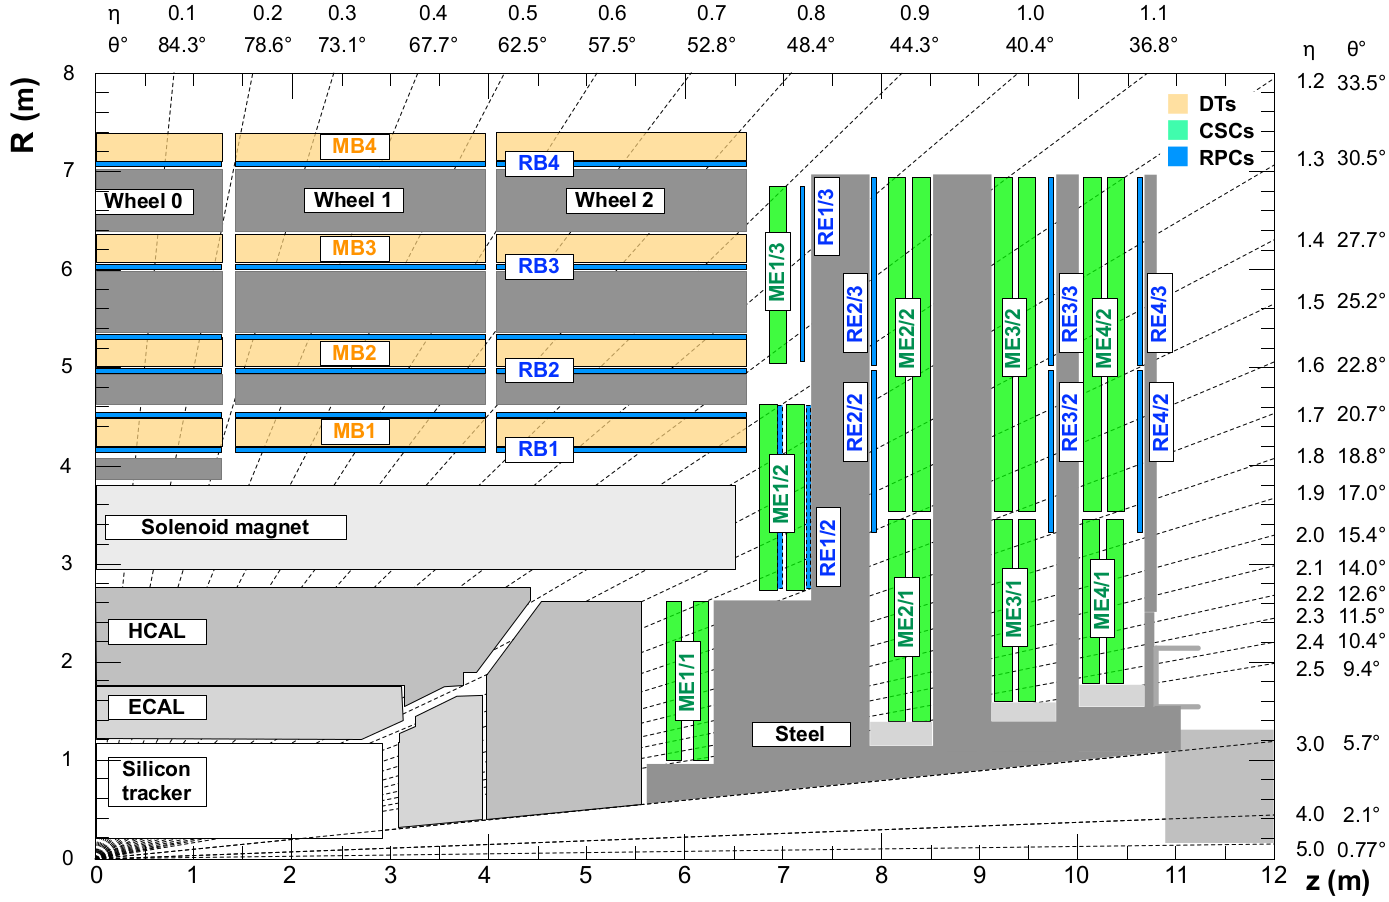
\includegraphics[width=0.8\textwidth]{Figures/Experiment/CMS/MuonSystem.png}
 \caption{Geometric view of one quadrant the CMS detector in the $r$-z plane. Each chamber of the muon system is shown in blue (RPC), green (CSC) and orange (DT). Figure taken from Ref.~\cite{CMSMuonFig}.}
 \label{fig:CMS_Muon}
\end{figure}

The DT detectors are used in the barrel region of the muon system ($|\eta| < 1.2$). A DT consists of a \SI{50}{\um}-diameter anode wire placed inside a rectangular tube connected to two cathode strips and filled with a gas mixture of $85\%$ of Ar and $15\%$ of $\text{CO}_{2}$. The layout of a DT cell is displayed on the left of \fig{fig:CMS_DT}. When a charged particle passes through a DT, it ionises the gas releasing electrons that are then detected in the anode wire. The DT system is composed of 172000 anode wires of \SI{2.4}{\m} length. There are four DT chambers in each of the five barrel wheels and twelve azimuthal sectors. In total, the fourth station contain 70 DT chambers and the first three stations contain 60 DT chambers each. Four layers, each containing up to 60 DTs, are grouped in units called SuperLayers (SL). The DT chambers of the three inner stations (outermost station) are made of three (two) SLs. The first and third SL, as shown on the right of \fig{fig:CMS_DT}, have their anode wires installed parallel to the $z$-axis to measure the bending in the transverse plane, while the anode wires of the second SL are placed orthogonal to the beam line to measure the position in the $z$-coordinate. The SLs of the fourth station only have anode wires parallel to the $z$-axis. The SLs measure the position and angle of the track segments with a precision of \SI{1.5}{\mm} and \SI{20}{\milli\radian}, respectively.

\begin{figure}[!htbp]
 \centering
 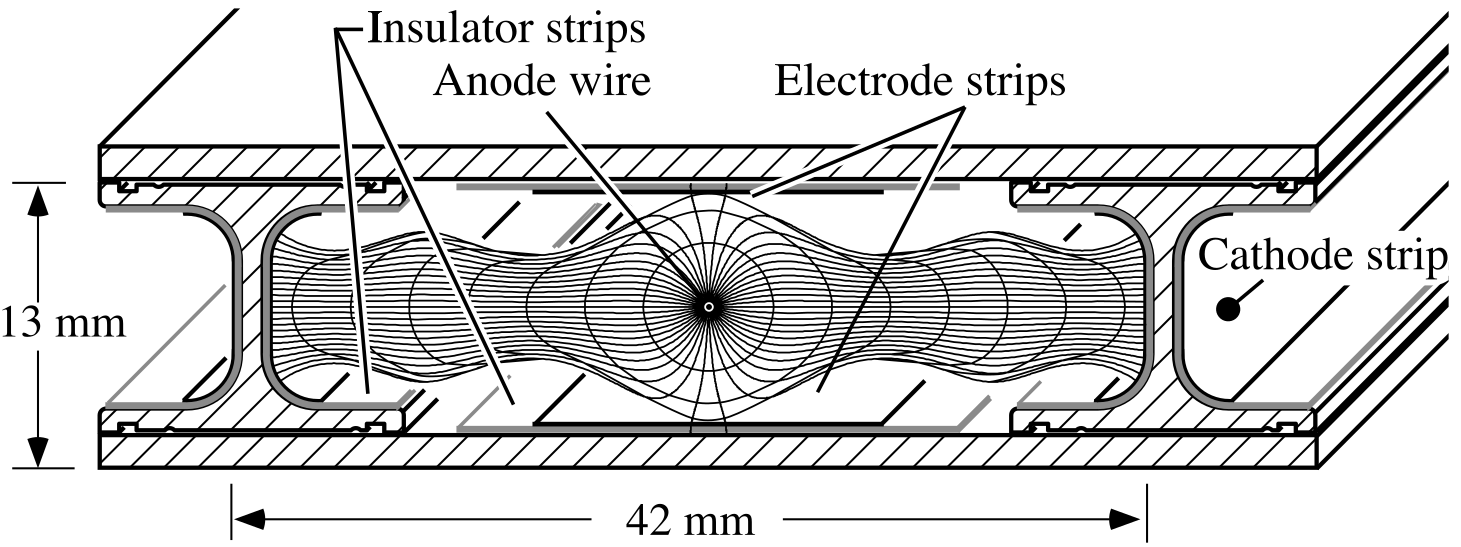
\includegraphics[width=0.53\textwidth]{Figures/Experiment/CMS/DT_2.png}
 %
 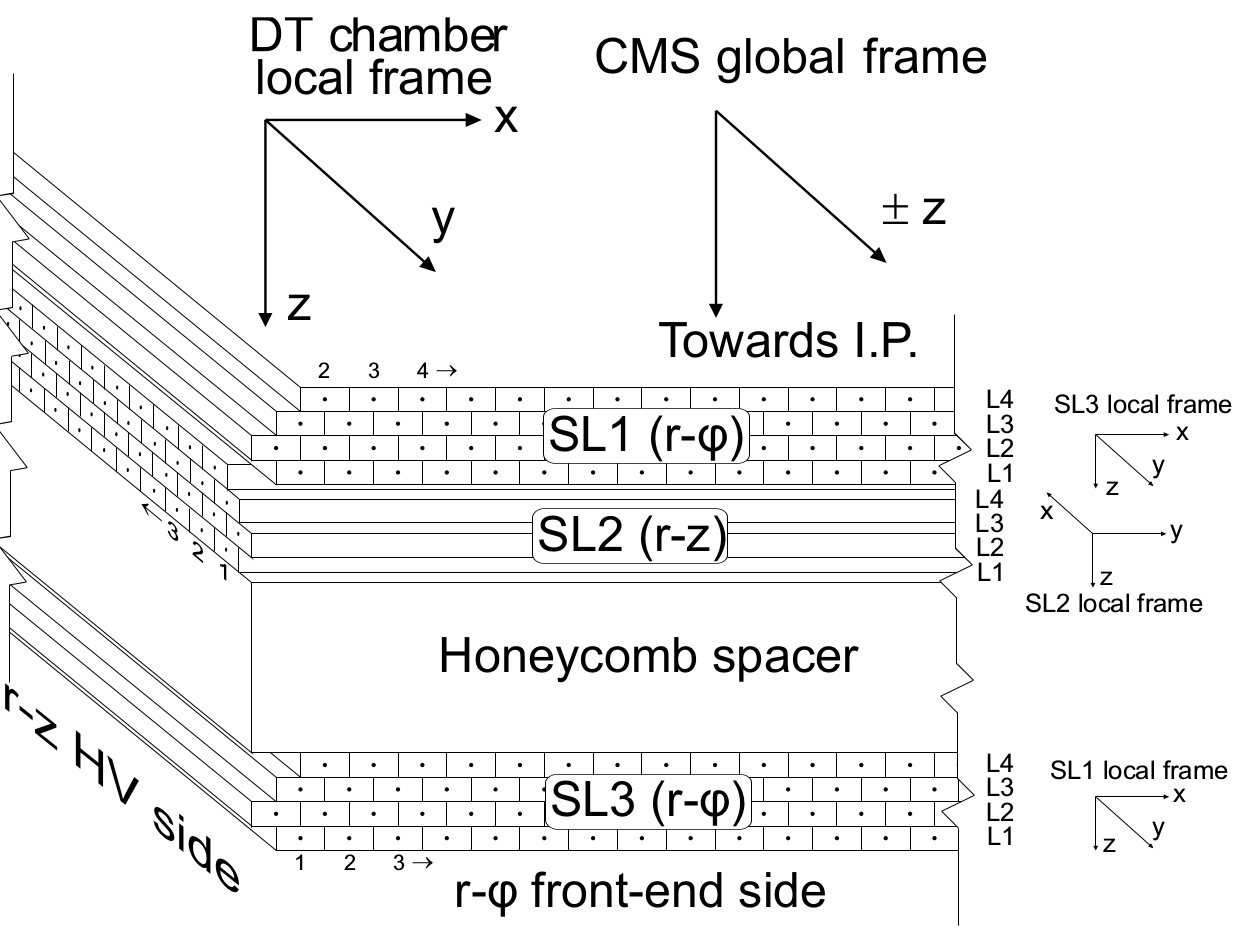
\includegraphics[width=0.43\textwidth]{Figures/Experiment/CMS/DT_1.png}
 \caption{Schematic layout of a DT cell (left) and a DT chamber (right). Figures taken from~\cite{CMSMuonDTFig}.}
 \label{fig:CMS_DT}
\end{figure}

Instead of DTs, the two endcap sections use 540 CSCs covering a pseudorapidity range $0.9 < |\eta| < 2.4$. The CSC system is designed to cope with the higher rate of particles and the large non-uniform magnetic field present in the forward region. A CSC is made of six anode wire planes crossed with seven cooper cathode strips within a gas mixture of $40\%$ Ar, $50\%$ $\text{CO}_{2}$, and $10\%$ $\text{CF}_{4}$, forming a multiwire proportional chamber. The CSCs are operated at \SI{3.6}{\kV} with a gas gain of $7{\times}10^{4}$, and are organised in chambers installed perpendicular to the beam pipe. The CSC chambers are trapezoidal and cover either \ang{10} or \ang{20} in $\phi$, and they overlap providing contiguous coverage in $\phi$. The cathode strips are milled in panels along constant $\Delta{\phi}$-width and provide measurements in the transverse plane, while the anode wires are placed azimuthally and measure the pseudorapidity of muons. The CSC system has a total of 266112 cathode-strip and 210816 anode-wire read-out channels. A schematic layout of a CSC is shown in \fig{fig:CMS_CSC}.

\begin{figure}[!htbp]
 \centering
 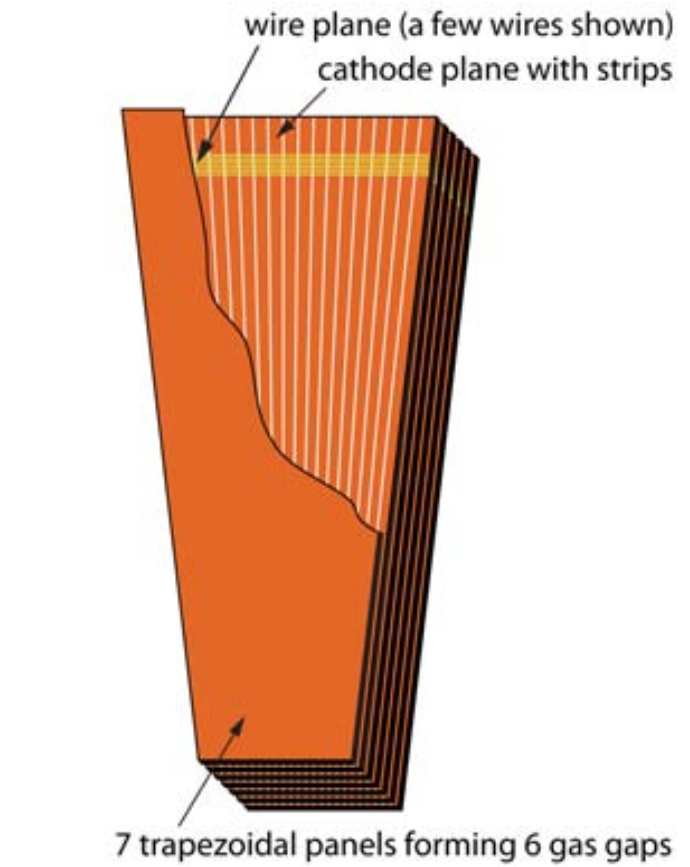
\includegraphics[width=0.4\textwidth]{Figures/Experiment/CMS/CSC.png}
 \caption{Schematic layout of a CSC. Figure taken from~\cite{CMS}.}
 \label{fig:CMS_CSC}
\end{figure}

To allow fast muon triggering, the barrel and endcap regions are complemented with RPC detectors. A RPC module consists of an anode plate parallel to a cathode plate, as shown in \fig{fig:CMS_RPC}. The  RPC plates are separated by a gap filled with a gas mixture of $96.2\%$ $\text{C}_{2}\text{H}_{2}\text{F}_{4}$, $3.5\%$ $i\text{C}_{4}\text{H}_{10}$ and $0.3\%$ $\text{SF}_{6}$, and operated in avalanche mode with read-out strips in between. There are 480 (576) RPC chambers in the barrel (endcap) region. Each RPC chamber consists of two or three modules of up to 96 strips each. Each RPC strip covers \ang{0.31} in $\phi$. The RPC chambers are organised in six coaxial cylinders in the barrel region and four rings in the endcaps, covering the pseudorapidity region up to $|\eta| = 1.9$. The innermost ring span \ang{20} in $\phi$ while the other rings span \ang{10}. The RPC modules are optimised for fast muon triggering by detecting ionising events faster than the time interval between two bunch crossings (\SI{25}{\ns}). They provide a good timing resolution but with a coarser spatial granularity compared to DTs and CSCs. The RPCs also allow to resolve ambiguities between tracks made from multiple hits in the muon chambers.

\begin{figure}[!htbp]
 \centering
 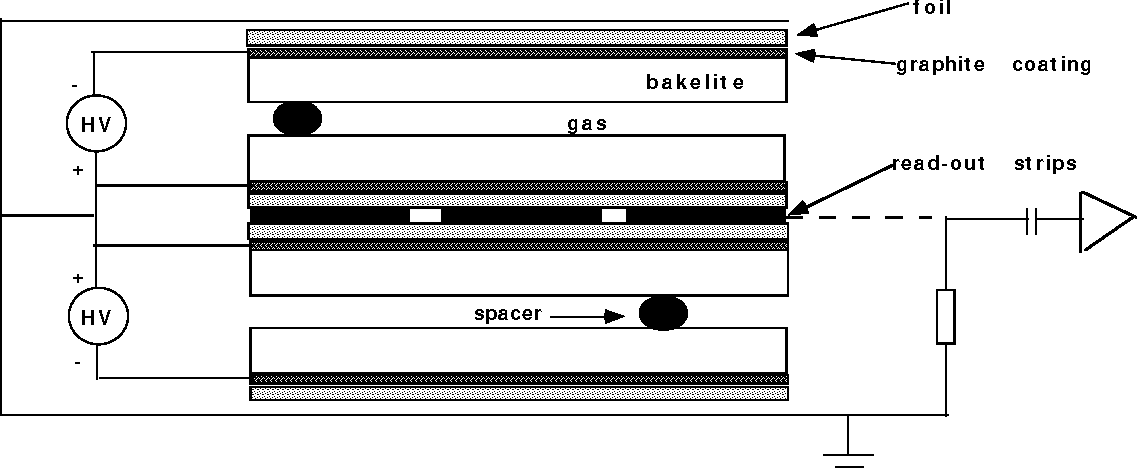
\includegraphics[width=0.49\textwidth]{Figures/Experiment/CMS/RPC_1.png}
 %
 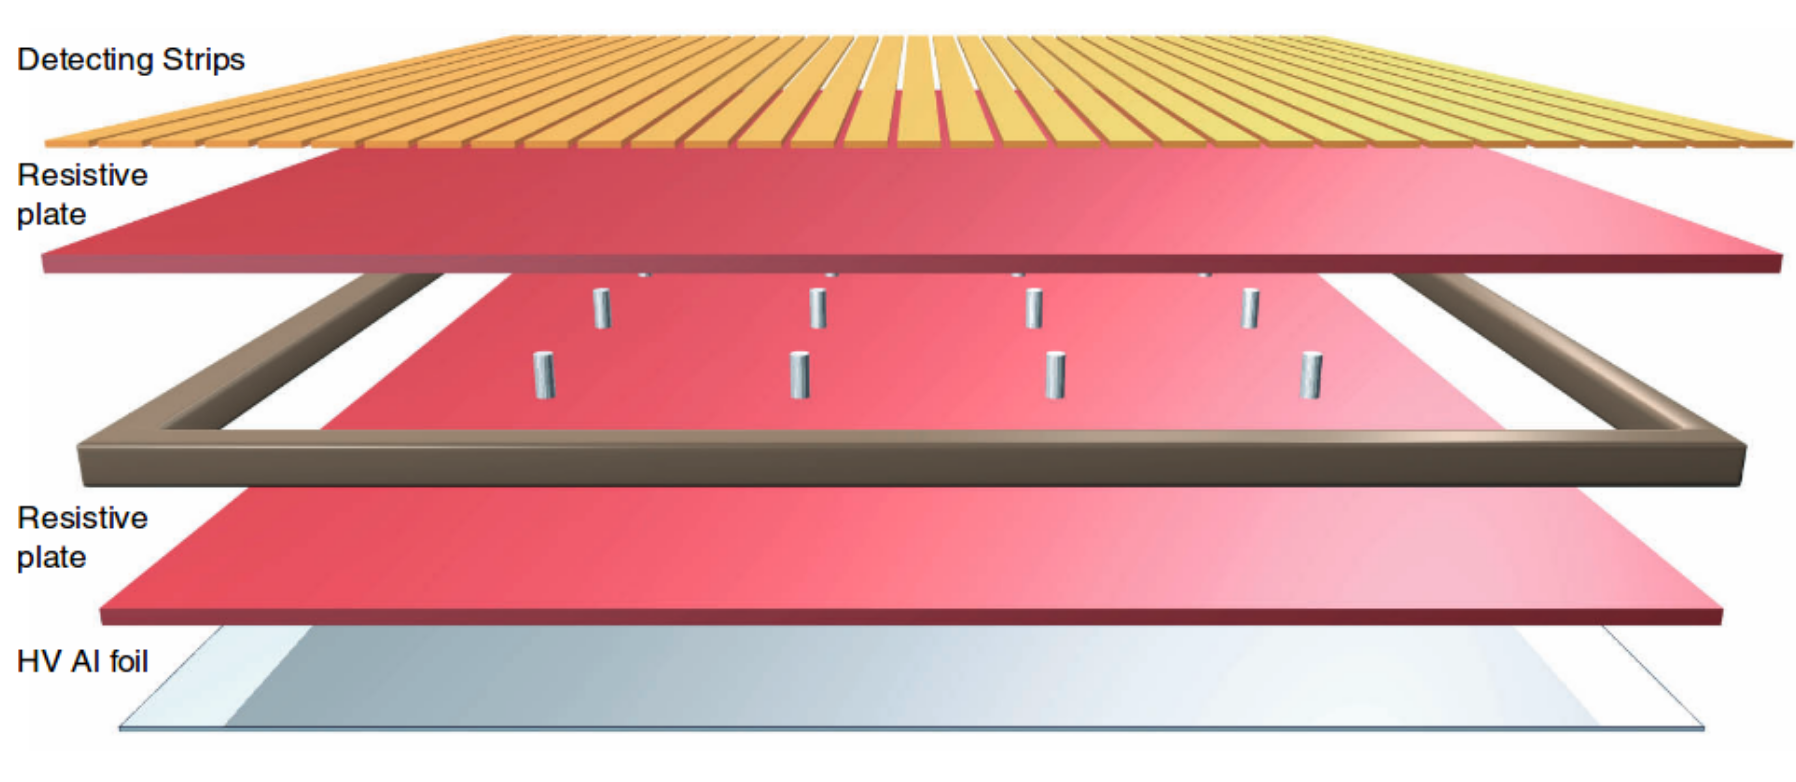
\includegraphics[width=0.49\textwidth]{Figures/Experiment/CMS/RPC_2.png}
 \caption{Cross section view (left)~\cite{CMSMuonRPCFig_1} and exploded view (right)~\cite{CMSMuonRPCFig_2} of a RPC module. }
 \label{fig:CMS_RPC}
\end{figure}



\subsection{Trigger system}\label{sec:Experiment_CMS_Trigger}

At LHC design conditions, the two beams crosses each IP every \SI{25}{\ns}, equivalent to a frequency of \SI{40}{\MHz}. Once a collision is recorded by CMS, all detector channels are read out and the data is sent to the CERN main computing farm, known as the Tier-0, to be further processed with the CMS SoftWare (CMSSW). However, the Tier-0 processing rate is limited by its CPU performance and storage capacity. As a result, the input rate of data transferred to the Tier-0 has to be kept below \SI{1}{\kHz} to avoid overflowing the computing centre.

To reach this goal, CMS has implemented a two-level trigger system designed to select events of interest for physics analysis. The first level, known as the Level-1 (L1) trigger, lowers the collision rate to an output rate of \SI{100}{\kHz} by filtering events using custom hardware. The next trigger level, called the High Level Trigger (HLT), is performed in a cluster of computers located in the CMS experimental cavern. The HLT software algorithms further reduce the data rate down the limit required by the Tier-0.

\subsubsection{Level-1 trigger}\label{sec:Experiment_CMS_Trigger_L1}

The L1 trigger system~\cite{CMSTrigger} is designed to handle the large collision rate of the LHC. To accomplish this goal, the L1 trigger is made of custom hardware modules optimised to process the events with a latency of less than \SI{4}{\us}. The L1 trigger is divided in two parts: the calorimeter and muon triggers.

The data from each subdetector are organised in units called Trigger Primitives (TP). The calorimeter TP are derived from the Trigger Towers (TT), each corresponding to a region of ${0.087}\times{0.087}$ in $\eta$-$\phi$ (represents $5\times{5}$ crystals in the ECAL). While for muons, a TP corresponds to a segment in either the DT or CSC systems. The information of the inner tracker is not used in the L1 trigger since the tracker data can not be currently read out within a bunch crossing time of \SI{25}{\ns}. As a result, the L1 calorimeter trigger cannot discriminate between electrons and photons. The output of the L1 muon and calorimeter triggers is combined in the L1 Global Trigger (GT), which then takes the final decision to either reject or accept the event.

The L1 trigger decision is determined according to a set of user-defined L1 trigger conditions. The L1 criteria are organised in a menu made of different algorithms which are programmed by the users and hard-coded in the firmware of a Field-Programmable Gate Array (FPGA). Some typical conditions used to define the L1 algorithms include setting a minimum \pt threshold or $\eta$ range on the L1 objects, or requiring events to have a given amount of L1 candidates. If an event passes the conditions of at least one of the L1 algorithms, the whole CMS detector is read out and the data is then sent to the HLT computers. The L1 menu is updated several times during data taking, to adapt to the changes in the LHC beam conditions and physics requirements.

In order to reduce the contribution from cosmic muons and also suppresses pre-firing from the calorimeters caused by particles interacting in the photomultipliers, the events processed by the L1 trigger  are required to be associated to a bunch crossing. The Beam Pick-up Timing eXperiment (BPTX) detectors, installed at a distance of $z = {\pm}\SI{175}{\meter}$ on each side of the IP, are used to select valid bunch crossings by checking for a coincidence of the signals on each side.

The L1 system underwent, between 2014 and 2015, an extensive upgrade that included a complete replacement of the electronics and the data acquisition system. The previous L1 trigger, used during LHC Run-1 and 2015, is referred in this manuscript as the legacy L1 trigger, while the L1 trigger deployed before the \pPb collision run in 2016, is called the upgraded L1 trigger.

\paragraph{Legacy L1 trigger.} The legacy L1 trigger~\cite{CMSTrigger} was used in CMS until the end of 2015, covering the entire LHC Run-1 and beginning of Run-2 data taking periods. The events from \Runpp and \RunPbPb collisions at $\sqrtsnn = \SI{5.02}{\TeV}$, in particular the data used for the charmonium analysis reported in \chp{sec:Charmonia}, were selected using the legacy L1 trigger. \fig{fig:L1TriggerLegacy} shows a diagram of the legacy L1 trigger system.

\begin{figure}[!htbp]
 \centering
 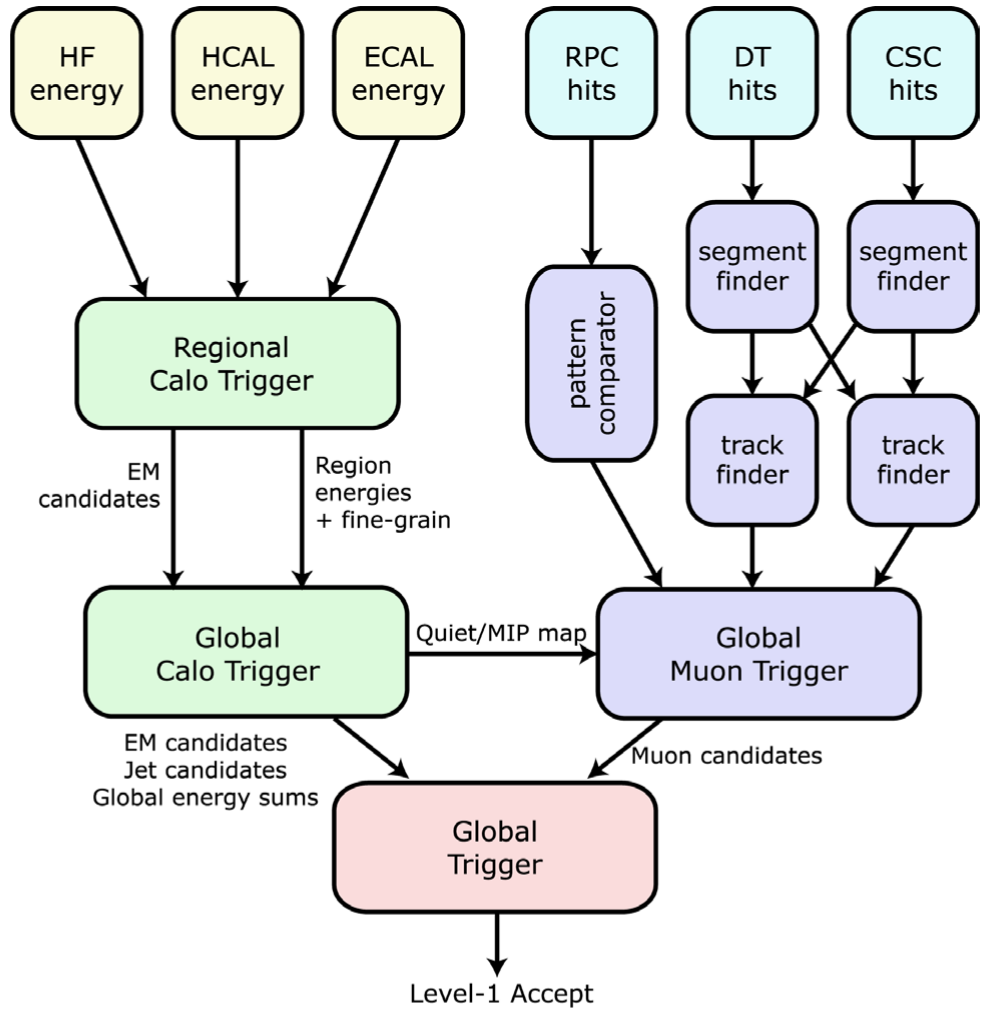
\includegraphics[width=0.6\textwidth]{Figures/Experiment/CMS/L1Trigger_Legacy.png}
 \caption{Diagram of the legacy L1 trigger of CMS. Figure taken from Ref.~\cite{L1TriggerLegacyFig}.}
 \label{fig:L1TriggerLegacy}
\end{figure}

In the legacy L1 trigger, the transverse energy \Et values are read out from each ECAL, HF and HCAL TT, and then sent to the Regional Calorimeter Trigger (RCT). The RCT processes the raw data and produces 72 electron-photon ($e/\gamma$) candidates (identified as energy clusters mainly deposited in the ECAL), computes the \Et in the HF region and derives 396 \Et sums of $4\times{4}$ TT regions. The Global Calorimeter Trigger (GCT) then receives the objects from the RCT and reconstructs jets and hadronic tau decays based on the regional \Et sums, sorts the $e/\gamma$ candidates according to their \Et, and computes global quantities such as the total \Et. Eight $e/\gamma$ candidates, eight jets, four tau candidates, the HF \Et, and the global quantities are then sent to the GT.

The legacy L1 muon trigger follows a detector-based design. The DT and CSC hit measurements are used by the front-end trigger electronics to reconstruct track segments in each muon station. Regional track finders (TF), one for each muon subsystem, sort the track segments and identify muons using pattern recognition algorithms. The hardware modules of the DT (CSC) TFs consists of 72 (12) Versa Module
Eurocard (VME) boards. The muon momentum is estimated based on the bending of the track along the magnetic field. The position of each muon detector hit is converted to $\eta$-$\phi$ coordinates using lookup tables derived from simulation. To cover the overlap region between the CSC and DT muon systems, the information of their TFs is combined. The RPC hits are directly sent to a pattern comparator trigger (PACT), which find muon candidates by comparing the RPC measurements to predefined patterns. Each muon TF determines the $\eta$-$\phi$ position and the \pt of the muon candidates, and also assigns a quality value based on the position and number of muon stations used to form the muon track.

On every bunch crossing, the CSC and DT TFs transfer, each one, four muon candidates to the Global Muon Trigger (GMT), while the RPC trigger sends eight muon candidates. The GMT then proceeds to merge the muon tracks if they have been identified by several muon subsystems, and assigns a three-bit quality code to the muon tracks depending on the information provided by each TF. All muon candidates are ranked in the GMT based on their quality code, and those with the same quality are then ranked based on their \pt. The four highest ranked candidates are then transferred to the GT. The quality bits assigned to the L1 muon candidates are: \begin{itemize}
  \setlength{\itemsep}{0pt}
  \setlength{\parskip}{0pt}
  \setlength{\parsep}{0pt}
  \item \textbf{Bits 0 to 4}: Represent empty, halo or very low quality muon tracks. Not used for physics.
  \item \textbf{Bit 5}: Muon candidate found by the DT or CSC TFs, but not confirmed by the RPC PACT.
  \item \textbf{Bit 6}: Muon candidate found by the RPC PACT, but not confirmed by the DT or CSC TFs.
  \item \textbf{Bit 7}: Muon candidate detected by the DT or CSC TFs, and also by the RPC PACT.
\end{itemize}

Finally, legacy GT takes the final L1 decision based on the information provided by the GMT and the GCT. It is able to evaluate up to 128 L1 algorithms.

\paragraph{Upgraded L1 trigger.} The upgraded L1 trigger system~\cite{L1_Stage2}, deployed in CMS at the beginning of 2016, was used during the data taking period of \RunpPb collisions at $\sqrtsnn = \SI{8.16}{\TeV}$, and thus for the \Wb-boson analysis reported in \chp{sec:WBoson}. A diagram of the upgraded L1 trigger system is shown in \fig{fig:L1TriggerStage2}.

\begin{figure}[!htbp]
 \centering
 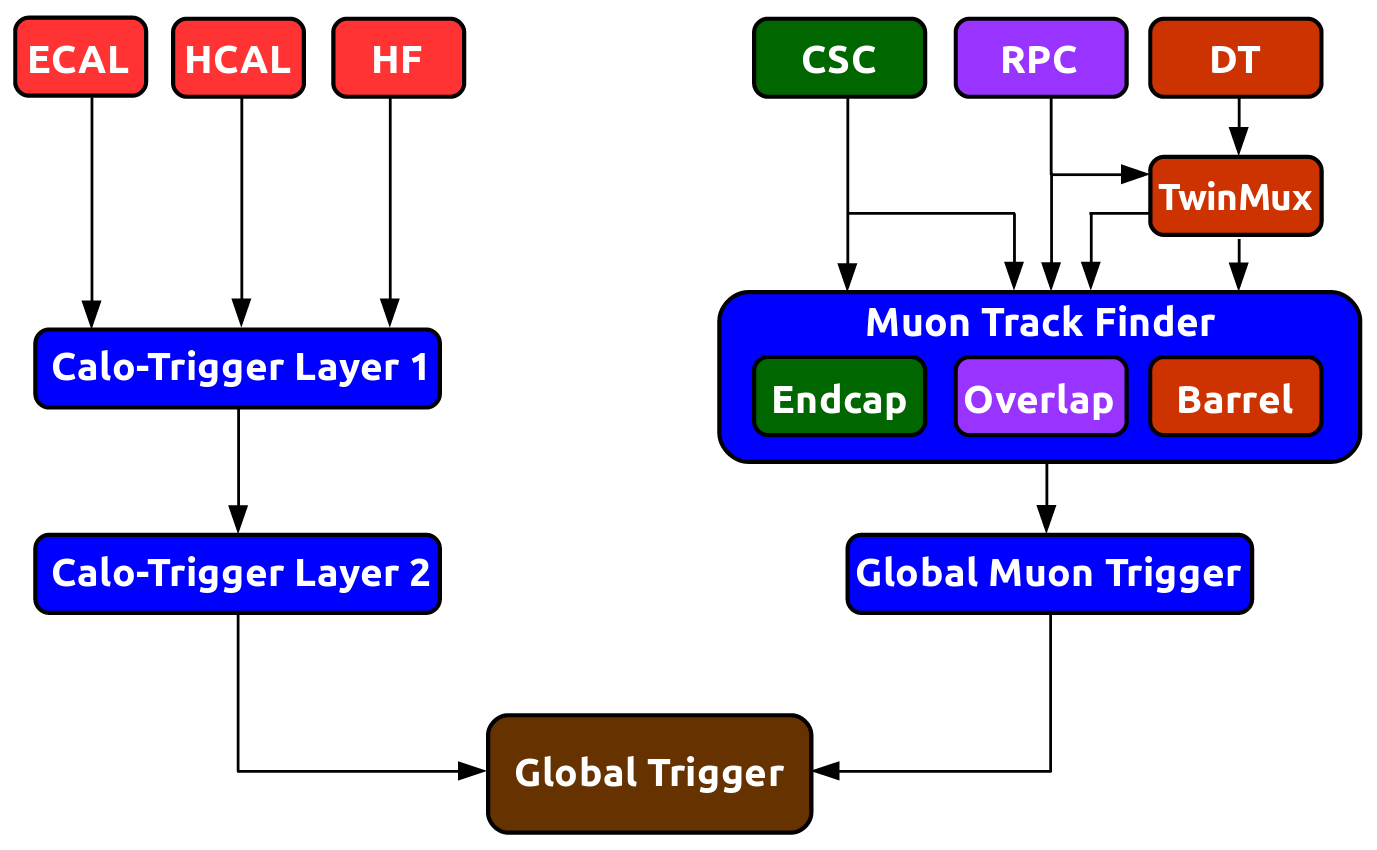
\includegraphics[width=0.8\textwidth]{Figures/Experiment/CMS/L1Trigger_Stage2.png}
 \caption{Diagram of the CMS L1 trigger used in 2016.}
 \label{fig:L1TriggerStage2}
\end{figure}

The electronic system of the upgraded L1 trigger consists of Xilinx Virtex-7 FPGAs mounted on Advanced Mezzanine Cards (AMC), designed according to the micro Telecommunications Computing Architecture ($\mu$TCA) standard. Compared to the VME standard employed in its predecessor, the $\mu$TCA standard provides higher scalability, flexibility and bandwidth. The communication links between the L1 boards were upgraded from copper serial links (limited to 1.2~\Gbs in the legacy L1 trigger) to high speed optical serial links capable of handling a bandwidth of up to 10~\Gbs.

The upgraded L1 calorimeter~\cite{Stage2L1Calorimeter} trigger is divided in two separate processing layers and its architecture follows a time-multiplexed trigger design (the data is splitted in bunch-crossing intervals instead of detector regions). The first layer (Layer-1) collects data from the calorimeter TTs with 36 trigger processor cards and then distributes all data for a given bunch crossing to one of the nine multi-purpose FPGAs of the second layer (Layer-2). The Layer-2 use the TT data to reconstruct $e/\gamma$ candidates, jets, and taus  (decaying to hadrons), and compute global energy quantities. Lookup tables are used to perform the shape pattern recognition and the energy calibration.

In the case of the L1 muon trigger~\cite{Stage2L1Muon}, its architecture is upgraded following a regional  approach. The data from the different muon subsystems are combined at an earlier stage than in the legacy trigger, and L1 muon tracks are reconstructed in three regions: barrel ($|\eta| < 0.8$), overlap ($0.8 < |\eta| < 1.25$), and endcap ($1.25 < |\eta| < 2.4$). The Endcap-Muon TF (EMTF) is designed to process the information from the CSC and RPC modules, however it only received data from the CSC system during 2016 since the RPC concentrator card was still been commissioning. The Barrel-Muon TF (BMTF) builds muon candidates using RPC hits and DT segments reconstructed in the central region. The transition area ($|\eta| \approx 1.04$) between the endcap and barrel sections is covered with the Overlap-Muon TF (OMTF), which takes into account the data from the three muon subsystems. The DT and RPC segments from the barrel region are collected by an intermediate layer called the TwinMux system, which concentrates data and distributes it to the BMTF and OMTF.

The upgraded GMT, referred as $\mu$GMT, receives up to 36 L1 muon candidates from each L1 muon TF. The $\mu$GMT sorts the muon tracks, removes duplicate muons found by different TFs and ranks the muon candidates by their \pt and track quality. The eight highest ranked L1 muon candidates are then sent to the GT. The information from the $\mu$GMT and the Layer-2 is used by the upgraded GT to evaluate up to 512 L1 algorithms and determine the final L1 decision.

\subsubsection{High level trigger}\label{sec:Experiment_CMS_Trigger_HLT}

The HLT is executed on a processor farm composed of an array of multi-core computers running a Linux-based operating system known as Scientific Linux. During 2016, approximately 20000 cores were employed to run the HLT~\cite{HLTHardware}. The HLT software is organised in readout, builder and filter units. The readout unit extracts the information from all CMS subsystems once an event passes the L1 trigger. The builder unit assembles the raw data provided by the readout unit to build detector segments, hits and clusters. The assembled data are subsequently sent to the filter unit which performs the reconstruction of physics objects and selects events for data analysis. The logic of the HLT reconstruction framework is similar to what is used in offline reconstruction but optimised to handle high input data rates ($\le\SI{100}{\kHz}$).

The structure of the HLT algorithms is organised in a set of processing steps, called HLT path, that runs the reconstruction and selection of events. Each HLT path consists of a sequence of processing units that runs in a predefined order and selects events based on user-defined conditions, such as requiring the presence of muons with \pt larger than a given threshold. Once an event has been accepted by the HLT, the CMS data is kept temporarily on disk and eventually sent to the Tier-0 computing facility for further offline processing. The HLT output rate is constrained by the size of the event data and the Tier-0 processing power. The average data size of an event in \Runpp collisions is around \SI{500}{\kilo\Bit}, while in central \RunPbPb collisions can reach values as large as \SI{3}{\mega\Bit} due to the higher particle multiplicity.

For the analyses presented in this manuscript, the data was triggered requiring the presence of identified muons. The reconstruction of muon candidates in the HLT is performed in two steps. The first one, referred as the Level-2 (L2), reconstructs muon tracks using data from the muon system only, while the next step, known as the Level-3 (L3), combines the information from both the inner tracker and the muon stations.

\paragraph{HLT L2 muon reconstruction.} The L2 muon algorithm starts by performing a local reconstruction of the muon detectors to determine the hits on each muon chamber. The CSC and DT hits are then combined to form segments, which are only kept if found near a L1 muon candidate. The muon segments are then recursively fitted with a Kalman Filter (KF) technique~\cite{KalmanFilter} to build the L2 muon tracks. Duplicate tracks are filtered by removing L2 muon tracks that share hits. The KF fit is constrained to the position of the IP to improved the \pt resolution of L2 muon candidates.

\paragraph{HLT L3 muon reconstruction.} The L3 muon reconstruction improves the momentum resolution by combining the measurements from the inner tracker and the muon chambers. The reconstruction of all tracks in the inner tracker (hereafter called tracker tracks) cannot be done at HLT due to timing constrains. Instead, a regional tracking is performed by only reconstructing tracker tracks close to the L2 muon candidates using three different seeding algorithms. In the first case, the seeds are defined by extrapolating the parameters (position and \pt) of the L2 muon tracks to the outer surface of the inner tracker. The second seeding procedure takes the extrapolated L2 muon tracks and updates their parameters with the hit information from the outermost layers of the silicon-strip tracker. And the third seeding algorithm uses segments from two pixel hits measured in consecutive layers found in a narrow $\eta$-$\phi$ region around each L2 muon track. Each seed is then used to build the tracker tracks with a KF fit. The reconstructed tracker and L2 muon tracks are propagated to a common surface, and then matched by comparing their goodness-of-fit $\chi^{2}$. If a L2 muon track and a tracker track is matched, the hits of both tracks are then combined and refitted to form the L3 muon track.


\subsection{Reconstruction}\label{sec:Experiment_CMS_Reconstruction}

The aim of the CMS event reconstruction algorithms is to build and identify the physics objects generated during the collision by processing the raw data recorded by the CMS detector. The reconstruction algorithms are implemented in CMSSW framework. Once an event is selected by the HLT, the detector information is then transferred to the Tier-0 computing centre and processed with CMSSW. The reconstruction software starts by building the hits, segments and clusters, measured in each of the CMS subdetectors. Afterwards, it process the detector information to form physics objects such as charged-particle tracks, muons, electrons, photons and jets. Global event quantities, like the missing transverse momentum (\ptmiss), are computed by combining the information from the different reconstructed objects. Only the reconstruction of muons and the \ptmiss are described hereafter, since they are the only objects used in the \Wb-boson and charmonium analyses presented in \chp{sec:WBoson} and \chp{sec:Charmonia}, respectively.


\subsubsection{Muon reconstruction}\label{sec:Experiment_CMS_Reconstruction_Muon}

Muon candidates are reconstructed in CMS using the information from the inner tracker and the muon system. Tracks formed in the muon system only are called \textit{standalone-muon} tracks, while those built in the inner tracker and matched to a hit in the muon system are referred to as \textit{tracker-muon} tracks. \textit{Global-muon} tracks are reconstructed by matching a tracker track with a standalone-muon track~\cite{MuonReco}. The three different types of muon tracks used in CMS are displayed in \fig{fig:MuonReco}.

\begin{figure}[!htbp]
 \centering
 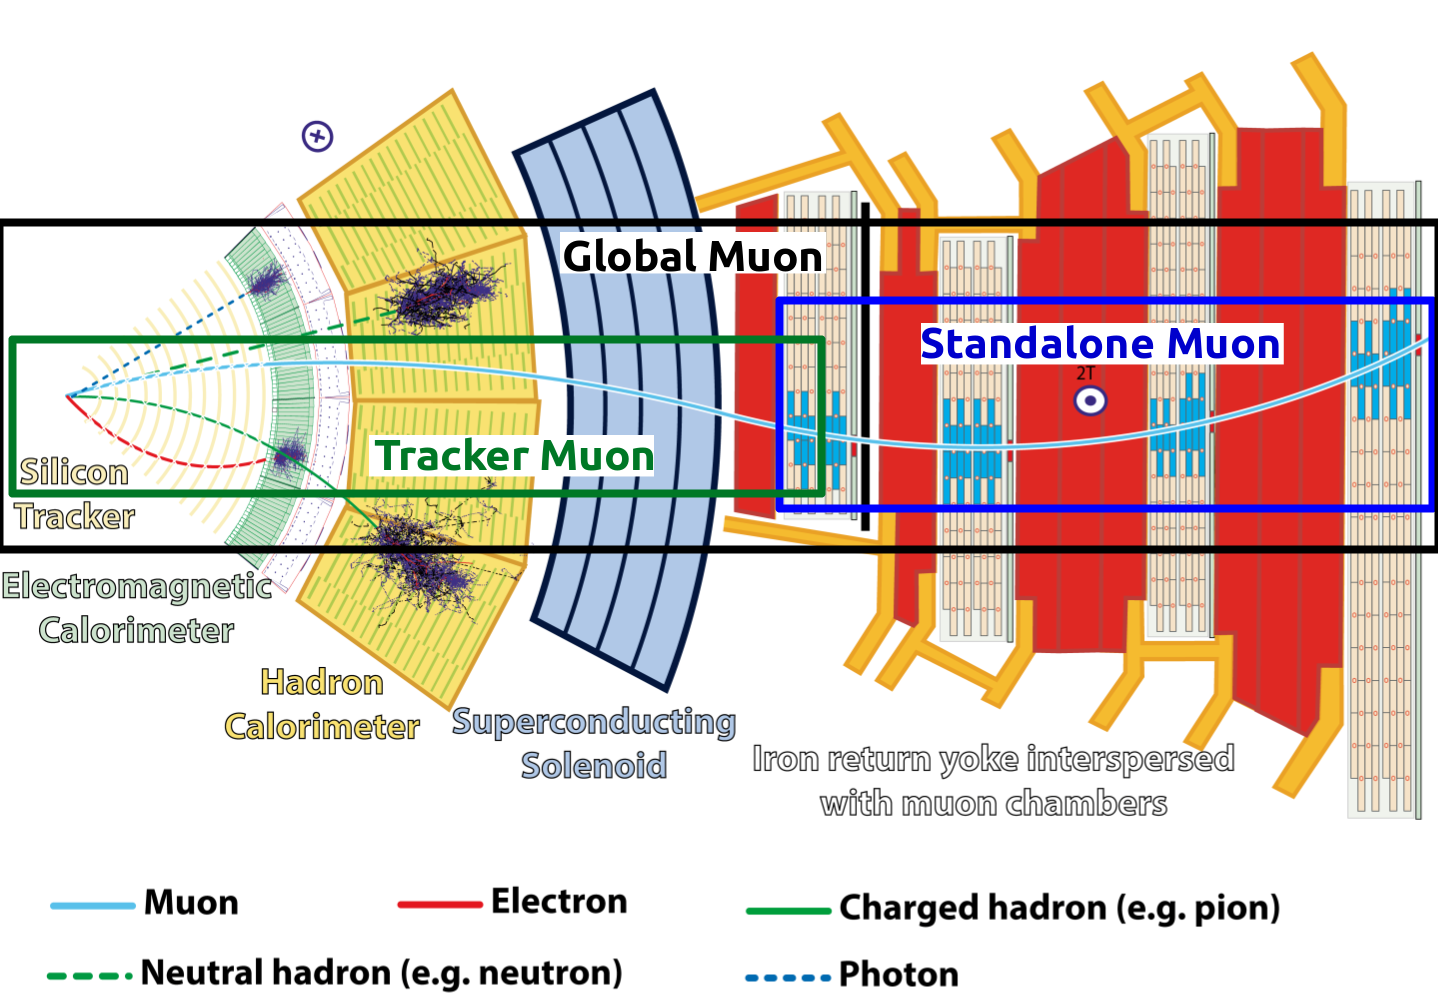
\includegraphics[width=0.8\textwidth]{Figures/Experiment/CMS/MuonReco.png}
 \caption{Cross section view of the CMS detector showing how particles interact interact in the CMS. The different types of muon tracks are indicated by boxes. Figure taken from Ref.~\cite{MuonRecoFig}. }
 \label{fig:MuonReco}
\end{figure}

\paragraph{Standalone muons.} The standalone muon reconstruction starts with the formation of segments made from a linear interpolation of the position of hits measured in the DT or CSC layers. Each track segment has an associated state vector representing its position, direction and \pt. The state vector of the segments built in the innermost muon station is used to seed the muon track fit.

In the barrel region, tracks are built by fitting the DT segments with a KF algorithm~\cite{KalmanFilter}, starting from the innermost muon chamber. Moreover, since the magnetic field in the endcap sections is not uniform, the hits of the CSC segments are used directly to perform the KF fit. The RPC hits are also included in the KF. In the case that no hits are found between muon layers, the state vector of the muon track is propagated to the next layer taking into account the magnetic field and the interaction of muons with the CMS detector material.

The track building procedure is iterated while progressing towards the outer muon chambers. The $\chi^{2}$ value between the detector hits and the position of the track projected onto the muon chambers is computed in each step. The hits with large $\chi^{2}$ values are excluded from the KF fit and the parameters of the track are updated accordingly. The track fit algorithm stops when it reaches the last muon station. Subsequently, the KF algorithm is performed backwards working from the outermost to the innermost muon chambers, completing the standalone-muon track. Finally, the standalone-muon tracks are extrapolated to the closest approach to the beam line and their position is required to be close to the IP.

\paragraph{Global muons.} The global muon reconstruction improves the momentum measurement by including the information from the inner tracker. The global muon tracking begins by propagating the standalone-muon tracks to the outer surface of the silicon-strip tracker, and a tracker layer consistent with the position of the propagated standalone muon then defines a common surface.

Tracker-track segments are built from pairs (triplets), made of two (three), hits reconstructed in adjacent inner-tracker layers. These segments are then employed to seed an iterative KF combinatorial track finder. The sophisticated tracking procedure runs ten different iterations. The first two iterations reconstruct low-\pt and high-\pt tracks seeded with pixel-hit triplets. The third iteration uses pixel-hit triplets to reconstruct tracks from secondary vertices displaced, within a radial distance R < 5 cm, from the primary vertex. The next iteration is meant to recover tracks with one or two missing hits by seeding with pixel-hit pairs instead. The fifth iteration build displaced tracks ($R < \SI{7}{\cm}$) seeded by triplets from pixel and strip hits. The following two iterations reconstruct very displaced tracks ($R < \SI{60}{\cm}$) seeded by strip-hit triplets. The eighth iteration aims to find tracks within the core of high-\pt jets seeded by pairs of pixel and strip hits. And the last two iterations build tracks seeded with hits and segments from the muon chambers, to improve the muon reconstruction efficiency. The hits associated to tracks formed in a given iteration are excluded in the subsequent iterations to avoid duplicating tracks. The rate of mis-reconstructed tracks is kept low in each step by applying a set of quality criteria on the goodness-of-fit $\chi^{2}$ and the number of hits used, and by requiring the tracks to be consistent with a charged-particle trajectory originating from the primary vertex.

The tracker track and the propagated standalone-muon track are matched in the common surface according to their \pt, position and direction measured in the common plane, and the hits from both tracks are then refitted to derive the ultimate global-muon candidate. If multiple global-muon tracks are found for the same standalone muon, the track with the best $\chi^{2}$ fit value is kept.

\paragraph{Tracker muons.} The tracker-muon candidates are built by propagating all tracker tracks with $\pt > 0.5~\GeVc$ and total momentum $p > 2.5$~\GeVc, outward to the innermost muon station.  The propagated track is then considered a tracker-muon track if it matches, along the transverse plane, at least one hit reconstructed in the inner muon chambers.


\paragraph{Tracking in \RunPbPb collisions.} A modified version of the tracker-track reconstruction was employed during \RunPbPb collisions at $\sqrtsnn = \SI{5.02}{\TeV}$, to cope with the large number of charged particles produced in central heavy-ion collisions. The tracking algorithm used to build the tracker tracks consists of seven iterations and is called Regional Iterative tracking (RegIt). Instead of using all pixel hits reconstructed in the inner tracker, RegIt performs a regional track reconstruction using only those hits found in a $\eta$-$\phi$ area around each standalone-muon track. The RegIt iterations follow the same logic as the standard tracking, excluding the three iterations corresponding to low-\pt, very displaced, and high-\pt jet tracks. In each iteration, tracks made with RegIt are required to have a $\pt > 0.8~\GeVc$ and at least eight hits, which is a tighter criteria compared to the standard track reconstruction.


\subsubsection{Missing transverse momentum reconstruction}\label{sec:Experiment_CMS_Reconstruction_MET}

Since neutrinos cannot be detected, their presence is inferred from the overall particle momentum imbalance in the transverse plane, known as missing transverse momentum (\ptmiss). The \ptmiss is defined as the magnitude of \ptvecmiss, which represents the negative vector sum of the transverse momentum of all particles identified by CMS in an event, as described in:

\begin{equation}
 \begin{aligned}
  \ptvecmiss &= -\sum_{\text{particles}}\ptvec \\
  \ptmiss &= \abs{\ptvecmiss}
 \end{aligned}
 \label{eq:MET}
\end{equation}

The Particle-Flow (PF) algorithm~\cite{PF_Reco} is used to identify the particles produced in a given event. The PF algorithm is optimised to reconstruct stable particles by taking into account the information from all CMS subdetectors. The algorithm determines the momentum of the reconstructed objects and classify them in five categories: electron, muon, photon, charged hadron and neutral hadron, as shown in \fig{fig:MuonReco}. The transverse momentum of all PF particles is used to compute the \ptmiss. The performance of the \ptmiss reconstruction in \Runpp collision data has been documented in~\cite{MET_Reco,MET_Reco_2}.


% END OF SECTION